\chapter{随机变量和分布函数}
\section{一维随机变量和一元分布函数}
\begin{definition}[随机变量]定义[2.1.1]
设 $(\Omega, \mathscr{F}, P)$ 是概率空间 (probability space)，
$X(\omega)$ 是 $\Omega$ 上的实值函数 (real-valued function)，
若对每个实数 $x$，均有
\[
\{\omega \mid X(\omega) < x\} \in \mathscr{F},
\]
则称 $X(\omega)$ 为 $(\Omega, \mathscr{F}, P)$ 上的随机变量 (random variable)。
\end{definition}
\begin{definition}[离散型随机变量]定义[2.1.2]
设 $X$ 是概率空间 $(\Omega, \mathscr{F}, P)$ 上的随机变量，若存在实数的有限集 (finite set) 或可列无穷集 (countable infinite set) $\{x_n\}$，使
\[
P\!\left(\bigcup_{n}\{X = x_n\}\right) = 1,
\]
则称 $X$ 为离散型随机变量 (discrete type random variable)。
\end{definition}
\begin{definition}[分布列]
设 $X$ 是概率空间 $(\Omega,\mathcal{F},P)$ 上的离散型随机变量，它以概率 $1$ 取值的集合为 $\{x_n\}$，当 $n\ne m$ 时，$x_n \ne x_m$。记
\[
p_n = P(X = x_n),
\]
则称 $\{p_n\}$ 为 $X$ 的\textbf{概率分布} (probability distribution) 或\textbf{分布列} (distribution sequence)。易知
\[
p_n \geq 0, \qquad \sum_{n=1}^{\infty} p_n = 1.
\]
\end{definition}
下面介绍几种常见的离散型随机变量及其概率分布。

\begin{enumerate}
  \item \textbf{单点分布}  
  设 $c$ 是实常数，若离散型随机变量 $X$ 有概率分布
  \[
  P(X=c)=1,
  \]
  则称 $X$ 服从取值于 $c$ 的\textbf{单点分布} (single-point distribution) 或\textbf{退化分布} (degenerate distribution)。

  \item \textbf{二项分布}  
  设 $n$ 是正整数，常数 $p\in(0,1)$，$q=1-p$。若离散型随机变量 $X$ 有概率分布
  \[
  P(X=k)=C_{n}^{\,k} p^{k} q^{\,n-k}, \qquad k=0,1,2,\dots,n, \tag{2.1.1}
  \]
  则称 $X$ 服从参数 $(n,p)$ 的\textbf{二项分布} (binomial distribution)，记作 $X\sim B(n,p)$。  

  由定理 1.5.4 知，二项分布的实际背景是 $n$ 次伯努利试验。
\end{enumerate}
\subsection{泊松分布}
\begin{dxtips}
    问题是一条路上，一个小时通过k辆车的概率是多少，把一个小时切成n段，n趋紧于无穷每一段时间只有通过一辆车和不通过两种情况。通过为p不通过为1-p，所以成了二项分布的问题。EX=np=$\lambda$历史数据,期望值，二项分布里面就是这样剩下1-p都是乘0的。期望不是平均。期望是加权和。
\end{dxtips}
\begin{theorem}[二项分布收敛到泊松分布的极限定理]定理[2.1.1]
对二项分布族 $\{B(n, p_n)\}$，其参数列 $\{p_n\}$ 满足
\[
\lim_{n \to \infty} n p_n = \lambda > 0,
\]
则对每个固定的非负整数 $k$，有
\[
\lim_{n \to \infty} b(k; n, p_n) = \frac{\lambda^k}{k!} e^{-\lambda}.
\]


\end{theorem}
\begin{corollary}[2.1.1]
设对每个正整数 $n$，$0 < p_n < 1$，如果对一切充分大的 $n$，有 $n p_n \equiv \lambda$，则二项分布的泊松定理成立。
\end{corollary}

\begin{proof}
这时，$\lim\limits_{n\to\infty} n p_n = \lambda$，所以，定理 2.1.1 的假设条件满足，因而结论成立。
\end{proof}

\begin{corollary}[2.1.2]
设 $0<p<1$，如果 $p$ 充分小，正整数 $n$ 充分大，$\lambda = np$，则对每个非负整数 $k\leq n$，有近似公式
\[
b(k;n,p)\approx \frac{\lambda^k}{k!} e^{-\lambda}. \tag{2.1.2}
\]
\end{corollary}

通常称公式 (2.1.2) 为二项分布的泊松近似公式 (approximation formula)。
\begin{proposition}[泊松分布由二项分布极限得到]
设随机变量 $X \sim B(n,p)$，令 $\lambda = np$。当 $n \to \infty,\; p \to 0$ 且 $\lambda$ 保持常数时，$X$ 的分布极限为泊松分布：
\[
P(X=k)=\frac{\lambda^{k}}{k!}\,e^{-\lambda}, \qquad k=0,1,2,\dots
\]
\end{proposition}
\begin{proof}
二项分布的分布律为
\[
P(X=k)=C_{n}^{\,k}\,p^{k}(1-p)^{\,n-k}.
\]
令 $p=\dfrac{\lambda}{n}$，则
\[
P(X=k)
= C_{n}^{\,k}\left(\frac{\lambda}{n}\right)^{k}\!\left(1-\frac{\lambda}{n}\right)^{n-k}
= \frac{n(n-1)\cdots(n-k+1)}{k!}\left(\frac{\lambda}{n}\right)^{k}\!\left(1-\frac{\lambda}{n}\right)^{n-k}.
\]

当 $n\to\infty$ 时，我们把极限拆成三个部分分别处理：

\begin{itemize}
 \item 组合系数部分


\[
\lim_{n \to \infty} \frac{C_n^k}{n^k} 
= \lim_{n \to \infty} \frac{n (n-1) \cdots (n-k+1)}{k! \, n^k}
= \lim_{n \to \infty} \frac{1}{k!} \cdot 
\left(1 - \tfrac{1}{n}\right)
\left(1 - \tfrac{2}{n}\right) 
\cdots 
\left(1 - \tfrac{k-1}{n}\right).
\]

由于每一项 $\left(1 - \tfrac{j}{n}\right) \to 1 \;(j=1,2,\dots,k-1)$，所以极限为
$
\frac{1}{k!}.
$

  \item 指数项部分
  \[
  \left(1-\frac{\lambda}{n}\right)^n.
  \]
  取对数：
  \[
  \ln\!\left(1-\frac{\lambda}{n}\right)^n = n \ln\!\left(1-\frac{\lambda}{n}\right).
  \]
  因为 $\ln(1+x)\sim x$（$x\to 0$），所以
  \[
  n \ln\!\left(1-\frac{\lambda}{n}\right) \sim -\lambda,
  \]
  从而
  \[
  \left(1-\frac{\lambda}{n}\right)^n \;\longrightarrow\; e^{-\lambda}.
  \]

  \item 负幂部分
  \[
  \left(1-\frac{\lambda}{n}\right)^{-k} \;\longrightarrow\; 1,
  \]
  因为 $\lambda/n \to 0$。
\end{itemize}

最后，把三部分合并：
\[
P(X=k)
=\lim_{n\to\infty} C_{n}^{\,k}\left(\frac{\lambda}{n}\right)^{k}\!\left(1-\frac{\lambda}{n}\right)^{n-k}
=\frac{\lambda^{k}}{k!}\,e^{-\lambda}.
\]

因此，当 $n\to\infty$ 且 $p=\lambda/n$ 时，二项分布 $B(n,p)$ 收敛到泊松分布 $\text{Poisson}(\lambda)$。
\end{proof}
\begin{definition}[泊松分布]
设 $\lambda$ 是正实数，若离散型随机变量 $X$ 有概率分布
\[
P(X=k)=\frac{\lambda^k}{k!}e^{-\lambda}, \qquad k=0,1,2,\dots, \tag{2.1.3}
\]
则称 $X$ 服从参数 $\lambda$ 的\textbf{泊松分布} (Poisson's distribution)，记作 $X\sim P(\lambda)$。
\end{definition}
\subsection{超几何分布}
\begin{definition}[超几何分布]
设 $N, M, n$ 是正整数，$M < N,\; n \leq N-M,\; l=\min(M,n)$。若离散型随机变量 $X$ 有概率分布
\[
P(X=k)=\frac{C_{M}^{\,k}\,C_{N-M}^{\,n-k}}{C_{N}^{\,n}}, 
\qquad k=0,1,2,\dots,l, \tag{2.1.4}
\]
则称 $X$ 服从\textbf{超几何分布} (hypergeometric distribution)，记作
\[
X \sim H(M,N,n).
\]

由例 1.2.6 知：若 $N$ 件产品中有 $M$ 件次品，$N-M$ 件正品，$M<N$。作不放回抽取，抽出 $n$ 件 ($n \leq N-M$)，以 $X$ 表示 $n$ 件中的次品数，则 $X \sim H(M,N,n)$。
\end{definition}
\begin{theorem}[2.1.2]
如果 $\displaystyle \lim_{N\to\infty}\frac{M}{N}=p$，则对任意固定的 $n,k$，有
\[
\lim_{N\to\infty}\frac{C_{M}^{\,k}\,C_{\,N-M}^{\,n-k}}{C_{N}^{\,n}}
= C_{n}^{\,k}\,p^{\,k}(1-p)^{\,n-k}. \tag{2.1.5}
\]
\end{theorem}

\begin{proof}
由组合恒等式
\[
\frac{C_{M}^{\,k}\,C_{\,N-M}^{\,n-k}}{C_{N}^{\,n}}
= C_{n}^{\,k}
\frac{M(M-1)\cdots(M-k+1)}{N^{k}}\;
\frac{(N-M)(N-M-1)\cdots\bigl(N-M-(n-k-1)\bigr)}{N^{\,n-k}}
\prod_{j=0}^{n-1}\frac{N}{N-j}.
\]
将各因子写成分式并取极限（$n,k$ 固定）：
\[
\frac{M-i}{N}\ \xrightarrow[N\to\infty]{}\ \frac{M}{N}\xrightarrow{}p,
\qquad
\frac{N-M-j}{N}\ \xrightarrow[N\to\infty]{}\ 1-\frac{M}{N}\xrightarrow{}1-p,
\qquad
\frac{N}{N-j}\xrightarrow[N\to\infty]{}1,
\]
其中 $i=0,1,\dots,k-1$，$j=0,1,\dots,n-k-1$。于是
\[
\frac{C_{M}^{\,k}\,C_{\,N-M}^{\,n-k}}{C_{N}^{\,n}}
\;\xrightarrow[N\to\infty]{}\;
C_{n}^{\,k}\,p^{\,k}(1-p)^{\,n-k}.
\]
证毕。
\end{proof}
 几何分布

若离散型随机变量 $X$ 有概率分布
\[
P(X=k)=p(1-p)^{k-1}, \quad k=1,2,\dots \tag{2.1.6}
\]
其中 $0<p<1$ 为常数，则称 $X$ 服从参数 $p$ 的几何分布（geometric distribution），记成
\[
X \sim G(p).
\]

几何分布是一种概率模型：在一个可进行无穷多次的伯努利试验中，事件 $A$ 在每次试验中出现的概率均为 $p$，将试验一个接一个地独立进行，设事件 $A$ 第一次出现时已进行了 $X$ 次试验，则 $X \sim G(p)$。
\begin{proposition}[几何分布的无记忆性]
若 $X \sim G(p)$，则对任意的正整数 $m,n$，总有
\[
P(X > n+m \mid X > n) = P(X > m).
\]
\end{proposition}

\begin{proof}
\begin{align*}
P(X > m+n \mid X > n) 
&= \frac{P(X > m+n,\; X > n)}{P(X > n)} \\[6pt]
&= \frac{P(X > m+n)}{P(X > n)} \\[6pt]
&= \frac{P(X \geq m+n+1)}{P(X \geq n+1)} \\[6pt]
&= \frac{\displaystyle \sum_{i=m+n+1}^\infty p(1-p)^{i-1}}
         {\displaystyle \sum_{i=n+1}^\infty p(1-p)^{i-1}} \\[10pt]
&= (1-p)^m \\[6pt]
&= \frac{p(1-p)^m}{1-(1-p)} \\[6pt]
&= P(X > m).
\end{align*}
证毕.
\end{proof}
该命题称为几何分布的“无记忆性（memoryless）”。其实际意义是：在进行 $n$ 次伯努利试验而事件 $A$ 未出现的条件下，再进行 $m$ 次伯努利试验而事件 $A$ 还未出现的概率，等于直接进行 $m$ 次伯努利试验而事件 $A$ 未出现的概率。它与在 $m$ 次伯努利试验之前是否进行过 $n$ 次伯努利试验无关。

无记忆性是几何分布的重要特征。
\subsection{负二项分布}
\begin{proposition}[6) 负二项分布]
 
若离散型随机变量 $X$ 有概率分布
\[
P(X=k) = \binom{k+r-1}{k} p^r (1-p)^k, \qquad k=0,1,2,\dots \tag{2.1.7}
\]
其中 $r$ 为固定的正整数，常数 $0<p<1$，则称随机变量 $X$ 服从参数为 $(r,p)$ 的   
\end{proposition}


\textbf{负二项分布}（negative binomial distribution），记作
\[
X \sim NB(r,p).
\]

负二项分布又称帕斯卡（Pascal）分布，它是几何分布的直接推广。  
同几何分布一样，负二项分布也可以由伯努利试验来定义。  
考虑伯努利试验，设事件 $A$ 在每次试验中出现的概率为 $p$，试验进行到 $A$ 第 $r$ 次出现时为止，记 $X$ 为 $A$ 第 $r$ 次出现前所做试验的次数，则
\[
X \sim NB(r,p).
\]

于是，$X \sim NB(1,p)$ 的充要条件为
\[
X+1 \sim G(p).
\]

容易推出：若 $X \sim NB(r,p)$，则存在独立同分布的随机变量 $X_1,X_2,\dots,X_r$，其分布均为 $G(p)$，使得
\[
X = X_1 + X_2 + \cdots + X_r - r.
\]

\section{2连续型随机变量}
\begin{definition}[连续型随机变量与概率密度函数]
定义2.14:设 $X$ 是概率空间 $(\Omega, \mathcal{F}, P)$ 上的随机变量，若存在实数集 $\mathbb{R}$ 上的非负实值函数 $f(x)$，使对任意实数 $a<b$，有
\[
P(a < X < b) = \int_a^b f(x)\,dx, \tag{2.1.8}
\]
则称 $X$ 为\textbf{连续型随机变量}（continuous random variable），称 $f(x)$ 为 $X$ 的\textbf{概率密度函数}（probability density function），有时也简称概率密度或密度。
\end{definition}
\begin{dxtips}
    叫密度是因为密度乘体积才有质量，(a,b)的区间就起到体积作用对。所以没有体积密度再大质量也是零P(X=a)永远是0
\end{dxtips}
\begin{remark}

概率密度函数 $f(x)$ 在某点 $a$ 处的高度，
并不反映随机变量 $X$ 取值为 $a$ 的概率。
但是，这个高度越大，
则 $X$ 取 $a$ \textbf{附近值} 的概率就越大。

\vspace{6pt}
\textcolor{green!70!black}{
密度曲线在某点的高度，反映了随机变量
在该点附近取值的集中程度。
}
\end{remark}
\begin{proposition}[只有小于号另一端默认负无穷]
定义 2.1.4 等价于下述定义：存在实数集 $\mathbb{R}$ 上的非负实值函数 $f(x)$，使对任意实数 $x$，有
\[
P(X < x) = \int_{-\infty}^x f(u)\,du. \tag{2.1.9}
\]
\end{proposition}
\begin{proposition}[概率密度函数的非唯一性]
设 $X$ 为连续型随机变量，$f(x)$ 为其概率密度函数。则概率密度函数的取值并非唯一确定。

\[
P(a<X<b)=\int_a^b f(x)\,dx
\]
仅依赖于 $f(x)$ 在积分意义下的值。若存在两个函数 $f_1(x),f_2(x)$ 满足
\[
\int_a^b f_1(x)\,dx=\int_a^b f_2(x)\,dx
\quad\text{对任意 }a<b,
\]
则它们表示同一概率分布。

因此，在概率论中，允许密度函数在\textbf{个别点（零测集）上不同}，而不影响分布的定义。通常取一个在连续点上尽量光滑、定义良好的函数作为代表。
\end{proposition}
\[
P(a \le X \le b)
= P(a < X \le b)
= P(a \le X < b)
= P(a < X < b).
\]边界上两个点不影响，因为测度是0
\begin{theorem}[概率密度函数的性质]
设 $X$ 为连续型随机变量，$f(x)$ 为其概率密度函数，则 $f(x)$ 必须满足以下三个基本性质：
\begin{enumerate}
  \item[\textbf{(1)}] \textbf{定义域：}
  \[
  f(x)\ \text{的定义域为整个实数轴 } (-\infty,+\infty)；
  \]
  \item[\textbf{(2)}] \textbf{非负性：}
  \[
  f(x)\ge 0,\quad \forall x\in\mathbb{R}；
  \]
  \item[\textbf{(3)}] \textbf{归一性：}
  \[
  \int_{-\infty}^{+\infty} f(x)\,dx = 1.
  \]
\end{enumerate}
以上三条性质共同确保 $f(x)$ 能正确描述随机变量 $X$ 在实数轴上的概率分布。
\end{theorem}
\subsection{均匀，指数分布}
\begin{proposition}[区间上的均匀分布]
设实数 $a<b$，若连续型随机变量 $X$ 的概率密度函数为
\[
f(x)=
\begin{cases}
\dfrac{1}{b-a}, & a \leq x \leq b, \\[6pt]
0, & \text{其他},
\end{cases} \tag{2.1.10}
\]
则称 $X$ 服从区间 $[a,b]$ 上的\textbf{均匀分布}（uniform distribution），记作
\[
X \sim U(a,b).
\]

容易知道，若 $a \leq c < d \leq b$，则
\[
P(c<X<d)=\frac{d-c}{b-a},
\]
即 $X$ 落在 $[a,b]$ 的子区间 $(c,d)$ 中的概率只依赖于区间长度 $(d-c)$，而不依赖于其位置。  
这一性质表明 $X$ 在 $[a,b]$ 的子区间中取值的概率具有均匀性。
\end{proposition}
\begin{dxtips}
    它的实际背景是： r.v X  在(a, b)中任意子集
内的概率与这个子集的长度成正比，即 X 在(a,b)
的每一位置取值机会均等.

\end{dxtips}
\begin{example}
某公共汽车站从上午 7 时起，每 15 分钟来一班车，即 
\textcolor{blue}{7:00，7:15，7:30，7:45} 等时刻有汽车到达此站。
如果乘客到达此站的时间 $X$ 是 7:00 到 7:30 之间的均匀随机变量，
试求他候车时间少于 5 分钟的概率。
\end{example}

\begin{solution}
以 7:00 为起点 $0$，以“分钟”为单位。

依题意， 
\[
X \sim U(0,30)
\]

其概率密度函数为：
\[
f(x)=
\begin{cases}
\dfrac{1}{30}, & 0<x<30,\\[6pt]
0, & \text{其它}.
\end{cases}
\]
等价地：到达后等车时间 $W$ 小于 5 分钟 
$\iff$ 乘客到达时刻 $X$ 落在每班车前的 5 分钟内。

在区间 $[0,30)$（以 7:00 为 0），班车在 $0,15,30$ 分钟发车，所以
\[
W < 5 \iff X \in (10,15)\ \cup\ (25,30).
\]

这两个区间总长度为 $5 + 5 = 10$ 分钟。因为 $X \sim U(0,30)$，
\[
P(W<5)
= \frac{\text{有利长度}}{\text{总长度}}
= \frac{10}{30}
= \boxed{\tfrac{1}{3}}.
\]

也可用积分表示：
\[
P(W<5)
= \int_{10}^{15}\frac{1}{30}\,dx
+ \int_{25}^{30}\frac{1}{30}\,dx
= \frac{1}{3}.
\]
\end{solution}
\begin{definition}[指数分布]
若随机变量 $X$ 具有概率密度函数
\[
f(x) =
\begin{cases}
\lambda e^{-\lambda x}, & x \ge 0, \\[6pt]
0, & x < 0,
\end{cases}
\qquad \lambda > 0,
\]
则称 $X$ 服从参数为 $\lambda$ 的\textbf{指数分布}。

常记为：
\[
X \sim E(\lambda).
\]

指数分布常用于描述事物的寿命，故又称为\textbf{寿命分布}。
\end{definition}
\begin{theorem}[指数分布的无记忆性]
若 $X$ 是连续型随机变量，则 $X$ 服从指数分布，
当且仅当 $X$ 具有\textbf{无记忆性（memoryless property）}：

\[
P(X > x + y \mid X > x) = P(X > y), 
\qquad \text{for any } x \ge 0,\ y \ge 0.
\]
\end{theorem}
\begin{remark}
    无记忆性意味着：

对指数分布而言，未来发生事件所需的时间与过去已经经过的时间无关。

例如：

如果一个灯泡的寿命服从指数分布，
那么“它已经亮了 10 小时”这件事不会影响“它再亮 5 小时的概率”。
\end{remark}
\subsection{正态分布}
\begin{definition}[正态分布（Normal Distribution）]
若随机变量 $X$ 的概率密度函数为
\[
f(x) = \frac{1}{\sigma\sqrt{2\pi}} 
       \exp\!\left[-\frac{(x-\mu)^2}{2\sigma^2}\right],
\qquad -\infty < x < +\infty,
\]
其中 $\mu$(均值期望) 和 $\sigma^2$(方差) 都是常数，
$\mu$ 任意，$\sigma > 0$，
则称 $X$ 服从参数为 $\mu$ 和 $\sigma^2$ 的\textbf{正态分布}。

记作：
\[
X \sim N(\mu, \sigma^2).
\]
\end{definition}
\begin{proposition}[正态分布的重要性与普遍性]
正态分布是概率论中最重要的分布之一，主要体现在以下几个方面：

\begin{enumerate}
  \item \textbf{普遍性：}
  正态分布是自然界和工程技术中\textcolor{red}{最常见的分布之一}。
  大量随机现象都服从或近似服从正态分布。
  实际上，如果一个随机指标受到诸多因素的影响，
  且每个因素的作用都较小且不具决定性，
  那么该随机指标往往服从或近似服从正态分布。
  
  \item \textbf{近似性：}
  正态分布可以作为许多分布的\textcolor{red}{近似分布}。
  这也是中心极限定理的理论基础之一。
  
  \item \textbf{优良性质：}
  正态分布具有许多其他分布所不具备的\textcolor{red}{良好数学性质}，
  如对称性、稳定性、可微性等。
\end{enumerate}

\vspace{1em}

\textbf{说明：}
正态分布能够刻画众多随机现象。
若随机变量受到多个相互独立的随机因素影响，
且每个因素的影响较小并具有加性特征，
则该随机变量服从正态分布。

\textbf{典型实例包括：}
\begin{itemize}
  \item 各种测量误差；
  \item 人的生理特征指标；
  \item 工厂产品的尺寸；
  
\end{itemize}
\end{proposition}
$\mu$ 决定图像的中心位置，$\sigma$ 决定图像中峰的陡峭程度，也即分布的集中程度。
\begin{definition}[正态分布与标准正态分布]
若随机变量 $X$ 的概率密度函数为
\[
f(x) = \frac{1}{\sigma \sqrt{2\pi}} 
e^{-\frac{(x-\mu)^2}{2\sigma^2}}, \qquad -\infty < x < \infty,
\]
其中 $\mu$ 为\textbf{均值}（期望），$\sigma > 0$ 为\textbf{标准差}，则称 $X$ 服从参数为 $\mu$ 与 $\sigma^2$ 的正态分布，记作
$
X \sim N(\mu, \sigma^2).
$

当 $\mu = 0, \sigma = 1$ 时，称该分布为\textbf{标准正态分布}，记作
$
X \sim N(0,1).
$
其概率密度函数为
\[
\varphi(x) = \frac{1}{\sqrt{2\pi}} e^{-\frac{x^2}{2}}, 
\qquad -\infty < x < \infty,
\]
其分布函数为
\[
\Phi(x) = \frac{1}{\sqrt{2\pi}} 
\int_{-\infty}^{x} e^{-\frac{t^2}{2}}\, dt.
\]

\textbf{标准化变换：}  
若 $X \sim N(\mu, \sigma^2)$，定义
$
Z = \frac{X - \mu}{\sigma},
$
则 $Z$ 服从标准正态分布：
$
Z \sim N(0,1).
$
此过程称为将一般正态分布变量\textbf{标准化}。
\end{definition}
\begin{theorem}
若随机变量 $X \sim N(\mu,\sigma^2)$，则对任意实数 $a<b$，有
\[
P(a<X<b) = \Phi\!\left(\frac{b-\mu}{\sigma}\right) - \Phi\!\left(\frac{a-\mu}{\sigma}\right). \tag{2.1.14}
\]
\end{theorem}
\begin{definition}[标准正态分布的分位点]
设随机变量 $X \sim N(0,1)$，对任意给定的 $0<\alpha<0.5$，称满足条件
\[
P(X > Z_\alpha) = \alpha
\]
的点 $Z_\alpha$ 为标准正态分布的上（或右侧）$\alpha$ 分位点（quantile, fractile）。

由标准正态分布上 $\alpha$ 分位点的定义，可知
\[
\Phi(-Z_\alpha) = \alpha, \qquad \Phi(Z_\alpha) = 1-\alpha.
\]

这在以后的数理统计中经常使用。
\end{definition}
\subsection{分布函数}
为了对离散型的和连续型的 r.v以及更广泛类型的r.v给出一种统一的描述方法，引进了分布函数的概念.random variable随机变量
\begin{definition}[分布函数]
设随机变量 $X$ 是概率空间 $(\Omega, \mathcal{F}, P)$ 上的实值随机变量（r.v.）。

定义函数
\[
F(x) = P(X < x), \qquad (-\infty < x < +\infty),
\]
称为随机变量 $X$ 的\textbf{分布函数}（distribution function）。

记作：
\[
X \sim F(x) \quad \text{或} \quad F_X(x).
\]

分布函数 $F(x)$ 的值表示随机变量 $X$ 取值小于 $x$ 的概率。
\end{definition}
\[
\text{由定义，对于任意实数 } x_1 < x_2, \quad
P\{x_1 \le X < x_2\} = P\{X < x_2\} - P\{X < x_1\}
= F(x_2) - F(x_1).
\]

因此，只要知道了随机变量 $X$ 的分布函数，
它的统计特性就可以得到全面的描述。
\begin{example}
已知随机变量 
\[
X \sim 
\begin{Bmatrix}
x_i &:& 0 & 1 & 2 \\[2pt]
p_i &:& \dfrac{1}{3} & \dfrac{1}{6} & \dfrac{1}{2}
\end{Bmatrix},
\]
求分布函数 \(F(x)\)。

\textbf{解：}
\[
F(x) = P(X < x).
\]

当 \(x \le 0\) 时，\(\{X < x\} = \varnothing\)，故 \(F(x) = 0。\)

当 \(0 < x \le 1\) 时，
\[
F(x) = P(X < x) = P(X = 0) = \frac{1}{3}.
\]
\begin{center}
\begin{tikzpicture}[scale=2,>=stealth]
  % 坐标轴
  \draw[->] (-0.3,0) -- (2.8,0) node[right] {$x$};
  \draw[->] (0,-0.1) -- (0,1.2) node[above] {$F(x)$};

  % 水平阶梯
  \draw[thick,blue] (-0.3,0) -- (0,0);
  \draw[thick,blue] (0,1/3) -- (1,1/3);
  \draw[thick,blue] (1,1/2) -- (2,1/2);
  \draw[thick,blue] (2,1) -- (2.8,1);

  % 开圆点 (不包含)
  \filldraw[white,thick] (1,1/3) circle(0.04);
  \filldraw[white,thick] (2,1/2) circle(0.04);

  % 实圆点 (包含)
  \filldraw[blue] (0,1/3) circle(0.04);
  \filldraw[blue] (1,1/2) circle(0.04);
  \filldraw[blue] (2,1) circle(0.04);

  % 标签
  \node[left] at (0,1/3) {$\tfrac{1}{3}$};
  \node[left] at (0,1/2) {$\tfrac{1}{2}$};
  \node[left] at (0,1) {$1$};
\end{tikzpicture}
\end{center}
\end{example}
\begin{proposition}[离散型随机变量的分布函数]
设离散型随机变量 $X$ 的分布律为
\[
P\{X = x_k\} = p_k, \quad k = 1, 2, 3, \ldots
\]
则其分布函数为
\[
F(x) = P(X < x) = \sum_{x_k < x} p_k.
\]
由于 $F(x)$ 表示 $X$ 取不大于 $x$ 的诸值 $x_k$ 的概率之和，
故又称 $F(x)$ 为\textbf{累计分布函数（cumulative distribution function, CDF）}。
\end{proposition}
\begin{example}
设连续型随机变量 $X$ 的概率密度函数为
\[
f(x) =
\begin{cases}
\dfrac{x}{2}, & 0 \le x \le 2, \\[4pt]
0, & \text{其它}.
\end{cases}
\]
求其分布函数 $F(x)$。
\end{example}

\begin{solution}
由定义，
\[
F(x) = P(X < x) = \int_{-\infty}^{x} f(t)\,dt.
\]

于是分情况讨论：
\[
F(x) =
\begin{cases}
0, & x < 0, \\[6pt]
\displaystyle \int_{0}^{x} \dfrac{t}{2}\,dt = \dfrac{x^{2}}{4}, & 0 \le x \le 2, \\[8pt]
\displaystyle \int_{0}^{2} \dfrac{t}{2}\,dt = 1, & x > 2.
\end{cases}
\]
\[
\boxed{F(x) =
\begin{cases}
0, & x < 0, \\[4pt]
\dfrac{x^{2}}{4}, & 0 \le x \le 2, \\[4pt]
1, & x > 2.
\end{cases}}
\]
\begin{center}
\begin{tikzpicture}[scale=2,>=stealth]
  % 坐标轴
  \draw[->] (-0.3,0) -- (2.8,0) node[right] {$x$};
  \draw[->] (0,-0.1) -- (0,1.2) node[above] {$F(x)$};

  % 曲线部分
  \draw[domain=0:2,smooth,variable=\x,blue,thick]
       plot ({\x},{(\x*\x)/4});

  % 线段
  \draw[thick,blue] (-0.3,0) -- (0,0);
  \draw[thick,blue] (2,1) -- (2.8,1);

  % 点
  \filldraw[blue] (0,0) circle(0.03);
  \filldraw[blue] (2,1) circle(0.03);

  % 标签
  \node[left] at (0,1) {$1$};
  \node[below] at (0,0) {$0$};
  \node[below] at (1,0) {$1$};
  \node[below] at (2,0) {$2$};
\end{tikzpicture}
\end{center}
\end{solution}
\begin{proposition}[连续型随机变量的分布函数]
若随机变量 $X$ 是连续型随机变量，且其概率密度函数为 $f(x)$，则
\[
F(x) = P(X < x) = \int_{-\infty}^{x} f(t)\,dt.
\]

因此，\textbf{分布函数是密度函数的变动上限定积分}。

连续型随机变量的概率密度函数 $f(x)$ 不一定连续，
但其分布函数 $F(x)$ 必连续。
\end{proposition}
\begin{theorem}[分布函数的性质]
设随机变量 $X$ 的分布函数为 $F(x)$，则 $F(x)$ 具有以下基本性质：

\begin{enumerate}[(1)]
  \item \textbf{非降性}：若 $x_1 < x_2$，则
  \[
  F(x_1) \le F(x_2).
  \]

  \item \textbf{极限性质}：
  \[
  F(-\infty) = \lim_{x \to -\infty} F(x) = 0, \qquad
  F(+\infty) = \lim_{x \to +\infty} F(x) = 1.
  \]

  \item \textbf{左连续性}：
  \[
  \lim_{x \to x_0^-} F(x) = F(x_0), \quad \forall\, x_0 \in \mathbb{R}.
  \]
\end{enumerate}
\end{theorem}
\begin{theorem}[判定分布函数的方法]
设 $F(x)$ 是定义在实数集 $\mathbb{R}$ 上的实函数，若 $F(x)$ 满足以下三个条件：

\begin{enumerate}[(1)]
  \item \textbf{非降性}：若 $x_1 < x_2$，则
  \[
  F(x_1) \le F(x_2);
  \]
  
  \item \textbf{极限性质}：
  \[
  F(-\infty) = \lim_{x \to -\infty} F(x) = 0, 
  \qquad
  F(+\infty) = \lim_{x \to +\infty} F(x) = 1;
  \]
  
  \item \textbf{左连续性}：
  \[
  \lim_{x \to x_0^-} F(x) = F(x_0), \quad \forall\, x_0 \in \mathbb{R}.
  \]
\end{enumerate}

则 $F(x)$ 必为某随机变量的分布函数。
\end{theorem}
\begin{proposition}[分布函数的凸组合性质]
若 $F_1(x)$ 与 $F_2(x)$ 均为分布函数，且 \(0 \le \lambda \le 1\)，则
\[
F(x) = \lambda F_1(x) + (1-\lambda) F_2(x)
\]
亦为分布函数。
\end{proposition}
\begin{proposition}[分布函数与随机变量的对应关系]
分布函数唯一确定随机变量的分布。

若分布函数 \( F(x) \) 是非降阶梯函数，
则由该分布函数所确定的随机变量必为\textbf{离散型随机变量}。
\end{proposition}
\begin{proposition}[分布函数与密度函数的关系]
若随机变量 \( X \) 为连续型，且 \( X \sim f(x) \)，则
\[
F(x) = P(X < x) = \int_{-\infty}^{x} f(t)\,dt.
\]
在 \( f(x) \) 的连续点处，有
\[
\frac{dF(x)}{dx} = f(x).
\]
\end{proposition}

\begin{proof}
由积分定义可得分布函数与密度函数互为反演关系。

反之，若分布函数 \( F(x) \) 为非降连续函数，且满足
\[
\forall x \le y,\quad F(y) - F(x) = \int_x^y F'(t)\,dt,
\]
则 \( F(x) \) 必为某连续型随机变量的分布函数，
其概率密度函数为
\[
f(x) = F'(x).
\]

\textbf{解释：}  
积分关系 \( F(x) = \int f(t)\,dt \) 表示“累积概率”，  
微分关系 \( f(x) = F'(x) \) 表示“概率密度”。  
二者互为逆运算，构成连续型随机变量的基本联系。
\end{proof}
\begin{proof}
其取值及分布律由分布函数的间断点完全决定：
\begin{itemize}
  \item 随机变量的取值为 \( F(x) \) 的间断点；
  \item 在每个间断点处的分布概率等于 \( F(x) \) 的跳跃度。
\end{itemize}

\textbf{说明：}  
分布函数的连续部分对应连续型随机变量；
而阶梯状的跳跃部分反映了离散型随机变量的概率集中位置。
\end{proof}
\begin{proof}
因为分布函数满足：
\begin{enumerate}
  \item 非降性：由 $F_1,F_2$ 的非降性保持；
  \item 极限性质：$F(-\infty)=0,\; F(+\infty)=1$；
  \item 左连续性：凸组合不改变连续性。
\end{enumerate}
故 $F(x)$ 仍为分布函数。

\medskip
\textbf{概率解释：}  
若随机变量 $X_1,X_2$ 的分布函数分别为 $F_1,F_2$，以概率 $\lambda$ 选取 $X_1$，以概率 $1-\lambda$ 选取 $X_2$，  
则所得混合随机变量 $X$ 的分布函数为
\[
F(x)=\lambda F_1(x)+(1-\lambda)F_2(x),
\]
即“分布函数的凸组合仍为分布函数”。
\end{proof}
\section{二维随机变量和二维分布函数}
\begin{definition}[二维随机变量的分布函数]
设 $(X,Y)$ 是概率空间 $(\Omega, \mathscr{F}, P)$ 上的二维随机变量，令
\[
F(x,y) = P(X < x,\, Y < y), \qquad -\infty < x,\, y < \infty,
\tag{2.2.1}
\]
则称二元函数 $F(x,y)$ 为二维随机变量 $(X,Y)$ 的\textbf{分布函数}，
或 $X$ 与 $Y$ 的\textbf{联合分布函数}（joint distribution function）。
\end{definition}
比如说打靶子，需要x，y都符合靶子内。
\begin{compare}[]
二维随机变量 $(X,Y)$ 的联合分布函数 
\[
F(x,y) = P(X < x,\, Y < y), \qquad -\infty < x, y < \infty.
\]
\tcblower
一维随机变量 $X$ 的分布函数
\[
F(x) = P(X < x), \qquad -\infty < x < \infty.
\]
\end{compare}
由定义，对任意实数 $x_1 < x_2,\, y_1 < y_2,$
\[
P\{\,x_1 \le X < x_2,\, y_1 \le Y < y_2\,\}
= F(x_2,y_2) + F(x_1,y_1) - F(x_1,y_2) - F(x_2,y_1).
\]

因此，只要知道了随机向量 $X$ 的分布函数，  
它的统计特性就可以得到全面的描述。
\begin{theorem}[二维分布函数的性质]
若 $F(x,y)$ 是二维随机变量 $(X,Y)$ 的分布函数，则有：
\begin{enumerate}[(1)]
\item $F(x,y)$ 分别是 $x,y$ 的单调不减函数；
\item $F(x,y)$ 分别是 $x,y$ 的左连续函数；
\item 任意固定 $y$，有 
\[
F(-\infty,y)=\lim_{x\to -\infty}F(x,y)=0;
\]
任意固定 $x$，有 
\[
F(x,-\infty)=\lim_{y\to -\infty}F(x,y)=0;
\]
且 
\[
F(+\infty,+\infty)=\lim_{x,y\to +\infty}F(x,y)=1;
\]
\item 对任意固定的实数对 $a_1<b_1,\, a_2<b_2$，有
\[
P(a_1\le X<b_1,\ a_2\le Y<b_2)
=F(b_1,b_2)-F(a_1,b_2)-F(b_1,a_2)+F(a_1,a_2).
\]
\end{enumerate}
\end{theorem}
\begin{theorem}\label{thm:2.2.2}
若二元实变实值函数 $F(x,y)$ 满足定理~2.2.1~中的~(1)--(4)，
则存在某概率空间上的一个二维随机变量，
其分布函数恰为 $F(x,y)$。
\end{theorem}
\begin{example}
把一枚均匀硬币抛掷三次，设 $X$ 为三次抛掷中正面出现的次数，
而 $Y$ 为正面出现次数与反面出现次数之差的绝对值。
求 $(X,Y)$ 的概率函数。
\end{example}
\begin{solution}
$(X,Y)$ 可取值
\[
(0,3),\ (1,1),\ (2,1),\ (3,3).
\]
由于每种结果概率为 $(1/2)^3=1/8$，则

\[
\begin{aligned}
P(X=0,Y=3)&=(1/2)^3=1/8,\\
P(X=1,Y=1)&=3(1/2)^3=3/8,\\
P(X=2,Y=1)&=3/8,\\
P(X=3,Y=0)&=1/8.
\end{aligned}
\]

于是联合分布列如下：
\[
\begin{array}{c|cc}
\hline
X \backslash Y & 1 & 3 \\ \hline
0 & 0 & 1/8 \\
1 & 3/8 & 0 \\
2 & 3/8 & 0 \\
3 & 0 & 1/8 \\ \hline
\end{array}
\]

\end{solution}

\begin{definition}\label{def:2.2.3}
若 $X$ 和 $Y$ 是概率空间 $(\Omega, \mathscr{F}, P)$ 上的两个一维离散型随机变量，  
则称 $(X,Y)$ 为 $(\Omega, \mathscr{F}, P)$ 上的\textbf{二维离散型随机变量}。  
若二元分布函数可以为某二维离散型随机变量的分布函数，  
则称此二元分布函数为\textbf{二维离散型分布函数}。
\end{definition}

\begin{definition}
设 $(X,Y)$ 是二维离散型随机变量，$X,Y$ 的概率分布分别为  
$\{P(X = x_i)\}$ 和 $\{P(Y = y_j)\}$，记  
\[
p_{ij} = P(X = x_i,\, Y = y_j),
\]
则称 $\{p_{ij}\}$ 为 $(X,Y)$ 的\textbf{概率分布}。

显然，$p_{ij} \ge 0,\ \sum_{i,j} p_{ij} = 1$；  
$(X,Y)$ 的分布函数为
\[
F(x,y) = \sum_{x_i < x,\, y_j < y} p_{ij}. \tag{2.2.4}
\]
\end{definition}
求密度函数之前先求分布函数
设二维随机向量 $(X,Y)$ 的分布函数为 $F(x,y)$，  
若存在二维实平面上的非负可积函数 $f(x,y)$，使得对任意一点 $(x,y)$，恒有
\[
F(x,y) = \int_{-\infty}^{x} \int_{-\infty}^{y} f(u,v)\,du\,dv,
\]
则称 $(X,Y)$ 为\textbf{连续型随机向量}，称 $f(x,y)$ 为 $(X,Y)$ 的\textbf{概率密度函数}，
称 $F(x,y)$ 为\textbf{连续型分布函数}。
不难得出，对连续型随机向量 $(X,Y)$，其概率密度与分布函数的关系如下：
\[
F(x,y) = \int_{-\infty}^{x} \int_{-\infty}^{y} f(u,v)\,du\,dv,
\]
并且在 $f(x,y)$ 的连续点，有
\[
f(x,y) = \frac{\partial^2 F(x,y)}{\partial x\,\partial y}.
\]
\begin{theorem}
若二维连续型随机变量 $(X,Y)$ 的联合概率密度为 $f$，  
则对于 $\mathbb{R}^2$ 的 Lebesgue 可测子集 $A$，有
\[
P\{(X,Y)\in A\} = \iint_{A} f(x,y)\,dx\,dy.
\]
\end{theorem}
\begin{example}
    

设 $(X,Y)$ 的概率密度为
\[
f(x,y)=
\begin{cases}
cy(2-x), & 0\le x\le 1,\ 0\le y\le x,\\[4pt]
0, & \text{其它.}
\end{cases}
\]
求：(1) 常数 $c$ 的值；(2) $P(X+Y<1)$。
\end{example}

\begin{solution}
(1) 由概率密度函数的性质
\[
\iint_{-\infty}^{+\infty} f(x,y)\,dx\,dy = 1,
\]
确定常数 $c$。

由于 $f(x,y)$ 在 $0\le x\le 1,\,0\le y\le x$ 上非零，
\[
\int_0^1\!\!\int_0^x cy(2-x)\,dy\,dx
= c\!\int_0^1 \!\left[\frac{x^2(2-x)}{2}\right]dx
= \frac{5c}{24} = 1,
\]
故
\[
\boxed{c = \tfrac{24}{5}}.
\]
\end{solution}
\begin{proposition}[均匀分布]
设 $G$ 是平面上的有界区域，其面积为 $A$。  
若二维随机变量 $(X,Y)$ 具有概率密度
\[
f(x,y)=
\begin{cases}
\dfrac{1}{A}, & (x,y)\in G,\\[6pt]
0, & \text{其它.}
\end{cases}
\]
则称 $(X,Y)$ 在 $G$ 上服从\textbf{均匀分布}。

换言之，随机变量取值落在 $G$ 内任一小区域 $B$ 的概率与 $B$ 的面积成正比，  
而与 $B$ 的形状及位置无关。于是称 $(X,Y)$ 在 $G$ 上服从均匀分布。
\end{proposition}
方差是协方差矩阵
\begin{proposition}[正态分布]
若二维随机变量 $(X,Y)$ 具有概率密度
\[
f(x,y)=
\frac{1}{2\pi\sigma_1\sigma_2\sqrt{1-\rho^2}}
\exp\!\left\{
-\frac{1}{2(1-\rho^2)}
\!\left[
\left(\frac{x-\mu_1}{\sigma_1}\right)^2
-2\rho\!\left(\frac{x-\mu_1}{\sigma_1}\right)\!\left(\frac{y-\mu_2}{\sigma_2}\right)
+\left(\frac{y-\mu_2}{\sigma_2}\right)^2
\right]
\right\},
\]
其中 $\mu_1,\mu_2,\sigma_1,\sigma_2,\rho$ 均为常数，且
\[
\sigma_1>0,\quad \sigma_2>0,\quad |\rho|<1,
\]
则称 $(X,Y)$ 服从参数为 $\mu_1,\mu_2,\sigma_1,\sigma_2,\rho$ 的\textbf{二维正态分布}，  
记作
\[
(X,Y)\sim \mathcal{N}(\mu_1,\mu_2,\sigma_1,\sigma_2,\rho).
\]
\end{proposition}
\begin{proposition}[边缘分布函数]
设随机向量 $(X,Y)$ 的联合分布函数为 $F(x,y)$。

\begin{enumerate}[(1)]
\item 关于 $X$ 的边缘分布函数定义为
\[
F_X(x)=\lim_{y\to +\infty} F(x,y),
\]
表示随机变量 $X$ 取值不超过 $x$ 的概率。

\item 关于 $Y$ 的边缘分布函数定义为
\[
F_Y(y)=\lim_{x\to +\infty} F(x,y),
\]
表示随机变量 $Y$ 取值不超过 $y$ 的概率。
\end{enumerate}

\noindent
由定义可知，联合分布函数与边缘分布函数之间存在如下关系：

\begin{itemize}
  \item 联合分布函数 \textbf{唯一确定} 边缘分布函数；
  \item 但边缘分布函数 \textbf{不能唯一确定} 联合分布函数，  
  即给定一组边缘分布函数，可能对应无穷多个不同的联合分布函数。
\end{itemize}

\noindent
换言之，联合分布函数蕴含了随机变量之间的\textbf{相关结构信息}，  
而边缘分布仅反映各自的分布特征。
\end{proposition}
\begin{remark}
当我们让 \(y \to +\infty\) 时，意味着：
\(Y\) 取值不再受任何限制（因为 \(Y \le y\) 总是成立）。

在概率意义上，这就等价于“不管 \(Y\) 取什么值”。  
换句话说：
因此：
\[
F_X(x)
= \lim_{y \to +\infty} F(x,y)
= P(X \le x)
\]
于是自然得到：
\[
F_X(x) = \lim_{y\to+\infty} F(x, y) = P(X \le x)
\]
\end{remark}

\begin{center}

    
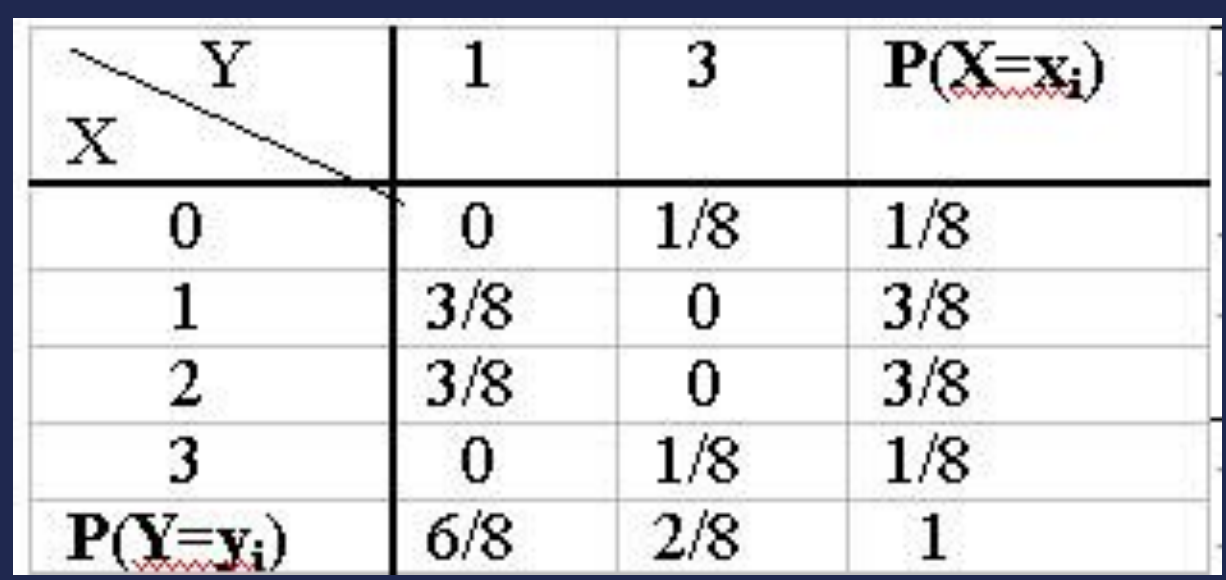
\includegraphics[width=0.5\linewidth]{image/截屏2025-10-17 09.23.43.png}

\end{center}



\begin{remark}
由定义可知，联合分布律与边缘分布律之间存在如下关系：

\begin{itemize}
  \item 联合分布律必然唯一地确定边缘分布律；
  \item 边缘分布律不能唯一地确定联合分布律，同一组边缘分布律可能对应无穷多种不同的联合分布律。
\end{itemize}
\end{remark}
\begin{theorem}[离散型随机变量的边缘分布律]
一般，对于离散型随机变量 $(X,Y)$，$X$ 和 $Y$ 的联合概率函数为
\[
P(X = x_i, Y = y_j) = p_{ij}, \qquad i, j = 1, 2, \ldots
\]

则 $(X,Y)$ 关于 $X$ 的边缘概率函数为
\[
P(X = x_i) = p_{i\bullet} = \sum_j p_{ij}, \qquad i = 1, 2, \ldots
\]

$(X,Y)$ 关于 $Y$ 的边缘概率函数为
\[
P(Y = y_j) = p_{\bullet j} = \sum_i p_{ij}, \qquad j = 1, 2, \ldots
\]
\end{theorem}
\begin{theorem}[连续型随机变量的边缘概率密度函数]
类似地，对于连续型随机变量 $(X,Y)$ 而言，  
如果 $X$ 和 $Y$ 的联合概率密度为
\[
f(x,y),
\]
则 $(X,Y)$ 关于 $X$ 的边缘概率密度函数为
\[
f_X(x) = \int_{-\infty}^{+\infty} f(x,y)\,dy,
\]
$(X,Y)$ 关于 $Y$ 的边缘概率密度函数为
\[
f_Y(y) = \int_{-\infty}^{+\infty} f(x,y)\,dx.
\]
\end{theorem}


\subsection*{随机变量的独立性}

\begin{definition}[随机变量的独立性]\label{def:independence}
设二维随机变量 $(X,Y)$ 的分布函数为 $F(x,y)$，
关于 $X$ 和关于 $Y$ 的边缘分布函数分别为 $F_X(x)$ 和 $F_Y(y)$。
如果对每组实数 $(x,y)$ 均有
\[
F(x,y) = F_X(x) F_Y(y),
\tag{2.3.1}
\]
则称 $X$ 与 $Y$ \textbf{相互独立}，简称\textbf{独立}。
\end{definition}
两个随机变量相互独立等价于它们的联合分布函数等于两个边缘分布函数的乘积，即
\[
F(x,y)=F(x,+\infty)\,F(+\infty,y).
\]

\begin{definition}[离散型随机变量的独立性]
若 $(X,Y)$ 是离散型随机变量，则独立性的定义等价于：

对于 $(X,Y)$ 的所有可能取值 $(x_i,y_j)$，都有
\[
P(X=x_i,\,Y=y_j)=P(X=x_i)\,P(Y=y_j),
\]
则称 $X$ 与 $Y$ \textbf{相互独立}。
\end{definition}
\begin{example}
从一副不含大小王的扑克牌中任取一张，记 $X$ 表示其点数，$Y$ 表示其花色（红或黑）。问：$X$ 与 $Y$ 是否独立？

\textbf{解：}  
点数取值 $X\in\{1,2,\dots,13\}$，花色取值 $Y\in\{r,b\}$，  
其中 $r$ 表示红色（红桃、方块），$b$ 表示黑色（黑桃、梅花）。

每种点数各有 $4$ 张牌，其中 $2$ 张红、$2$ 张黑。

故对任意 $i\in\{1,2,\dots,13\}$，$j\in\{r,b\}$，
\[
P(X=i,\,Y=j)=\frac{2}{52}=\frac{1}{26}.
\]

求边缘分布：
\[
P(Y=j)=\sum_i P(X=i,Y=j)=\frac{26}{52}=\frac{1}{2},
\qquad
P(X=i)=\sum_j P(X=i,Y=j)=\frac{4}{52}=\frac{1}{13}.
\]

检验独立性：
\[
P(X=i,\,Y=j)=\frac{1}{26}=\frac{1}{13}\cdot\frac{1}{2}=P(X=i)\,P(Y=j).
\]

因此，
\[
\boxed{X\text{ 与 }Y\text{ 相互独立.}}
\]
\end{example}
\begin{definition}[连续型随机变量的独立性]
若 $(X,Y)$ 是连续型随机变量，联合概率密度函数为 $f(x,y)$，
则 $X$ 与 $Y$ 相互独立当且仅当对任意的 $x,y$，
\[
f(x,y)=f_X(x)\,f_Y(y),
\]
其中 $f_X(x)$、$f_Y(y)$ 分别是 $X$ 与 $Y$ 的边缘密度函数。

“几乎处处成立” 的含义是：在平面上除去面积为零的集合外，该等式处处成立。
\end{definition}
\begin{example}
设 $(X,Y)$ 的联合概率密度为
\[
f(x,y)=
\begin{cases}
2, & 0<x<y<1,\\[4pt]
0, & \text{其他}.
\end{cases}
\]
问：$X$ 与 $Y$ 是否独立？

\textbf{解：}
先求边缘密度。

对 $X$：
\[
f_X(x)=\int_x^1 2\,dy = 2(1-x),\qquad 0<x<1.
\]

对 $Y$：
\[
f_Y(y)=\int_0^y 2\,dx = 2y,\qquad 0<y<1.
\]

检验独立性：
若 $X$、$Y$ 独立，则应有 $f(x,y)=f_X(x)f_Y(y)$。
然而在区域 $0<x<y<1$ 内，
\[
f_X(x)f_Y(y)=2(1-x)\cdot 2y = 4y(1-x)\ne 2=f(x,y),
\]
因此存在面积不为 $0$ 的区域使等式不成立。

故 $X$ 与 $Y$ \textbf{不独立}。
\end{example}















\subsection{条件分布}
\begin{definition}[离散型随机变量的条件分布]
设 $(X,Y)$ 是二维离散型随机变量。对于固定的 $j$，若 $P(Y=y_j)>0$，则称
\[
P(X=x_i\mid Y=y_j)
=\frac{P(X=x_i,Y=y_j)}{P(Y=y_j)}
=\frac{p_{ij}}{p_{\cdot j}},\qquad i=1,2,\dots
\]
为在 $Y=y_j$ 条件下随机变量 $X$ 的\textbf{条件概率分布律}或\textbf{条件分布函数}。
\end{definition}
\begin{example}
一射手进行射击，命中目标的概率为 $p\in(0,1)$。射击进行到命中目标两次为止。
记 $X$ 为\emph{首次命中}所对应的射击次数，$Y$ 为\emph{总射击次数}。
求 $(X,Y)$ 的联合分布及条件分布。
\end{example}

\begin{solution}
设每次射击独立，命中概率为 $p$、脱靶概率为 $q=1-p$。

\medskip\noindent
\textbf{(1) 支持集与联合分布 $P(X=k,Y=n)$}。  
必须 $n\ge 2$ 且 $1\le k\le n-1$。事件 $\{X=k,Y=n\}$ 等价于
\[
\underbrace{F\cdots F}_{k-1}\ S\ \underbrace{F\cdots F}_{n-k-1}\ S,
\]
即前 $k-1$ 次均脱靶，第 $k$ 次首次命中，随后直到第 $n-1$ 次全脱靶，第 $n$ 次第二次命中。  
故
\[
P(X=k,Y=n)=q^{\,k-1}\,p\;q^{\,n-k-1}\,p
= p^{2}q^{\,n-2},\qquad n\ge 2,\;1\le k\le n-1.
\]
（可见在给定 $n$ 时，对所有 $k=1,\dots,n-1$ 概率相同。）

\medskip\noindent
\textbf{(2) 边缘分布。}

\emph{总射击次数 $Y$：}  
\[
P(Y=n)=\sum_{k=1}^{n-1} P(X=k,Y=n)=(n-1)p^{2}q^{\,n-2},
\qquad n=2,3,\dots
\]
这是 $r=2$ 的负二项分布。

\emph{首次命中时刻 $X$：}  
\[
P(X=k)=q^{\,k-1}p,\qquad k=1,2,\dots
\]
这是几何分布（首中时刻）。

\medskip\noindent
\textbf{(3) 条件分布。}

\emph{给定 $Y$ 时 $X$ 的条件分布：}
\[
P(X=k\mid Y=n)
=\frac{P(X=k,Y=n)}{P(Y=n)}
=\frac{p^{2}q^{\,n-2}}{(n-1)p^{2}q^{\,n-2}}
=\frac{1}{n-1},
\quad k=1,\dots,n-1.
\]
即在给定总次数 $n$ 的条件下，首次命中时刻在 $\{1,\dots,n-1\}$ 上\textbf{均匀分布}。

\emph{给定 $X$ 时 $Y$ 的条件分布：}
\[
P(Y=n\mid X=k)
=\frac{P(X=k,Y=n)}{P(X=k)}
=\frac{p^{2}q^{\,n-2}}{q^{\,k-1}p}
= p\,q^{\,n-k-1},
\quad n=k+1,k+2,\dots
\]
即在首次命中于第 $k$ 次后，直到第二次命中所需的附加射击数为\textbf{几何分布}，$Y-k\sim\mathrm{Geom}(p)$（取值 $1,2,\dots$）。

\medskip
综上，联合分布、边缘分布与条件分布如上所示。
\end{solution}
\begin{theorem}[条件概率密度函数]
设随机变量 $X,Y$ 的联合概率密度为 $f(x,y)$，  
边缘概率密度分别为 $f_X(x),f_Y(y)$。

若 $f_X(x)>0$，则在 $X=x$ 的条件下，  
$Y$ 的条件概率密度函数为
\[
f_{Y|X}(y|x)=\frac{f(x,y)}{f_X(x)}.
\]

同样，对一切使 $f_Y(y)>0$ 的 $y$，  
已知 $Y=y$ 时，$X$ 的条件概率密度函数为
\[
f_{X|Y}(x|y)=\frac{f(x,y)}{f_Y(y)}.
\]
\end{theorem}
\begin{remark}
条件分布与条件密度的性质
\begin{itemize}
  \item 条件分布函数也满足分布函数的一切性质；
  \item 条件概率密度也满足概率密度的一切性质。
\end{itemize}

因此，对任意区间 $A$，
\[
P(X \in A \mid Y = y)
= \int_{A} f_{X|Y}(x \mid y)\,dx .
\]
\end{remark}
\begin{example}
设 \((X,Y)\) 的联合概率密度为
\[
f(x,y)=
\begin{cases}
\dfrac{e^{-x/y}e^{-y}}{y}, & 0<x<\infty,\ 0<y<\infty,\\[4pt]
0,& \text{其它}.
\end{cases}
\]
求 \(P(X>1\,|\,Y=y)\)。
\begin{solution}
先求边缘密度 \(f_Y(y)\)：
\[
f_Y(y)=\int_{0}^{\infty} f(x,y)\,dx
      =\int_{0}^{\infty}\frac{e^{-x/y}e^{-y}}{y}\,dx
      =\frac{e^{-y}}{y}\int_{0}^{\infty}e^{-x/y}\,dx
      =\frac{e^{-y}}{y}\,y\int_{0}^{\infty}e^{-u}\,du
      =e^{-y},\quad y>0.
\]
故条件密度
\[
f_{X|Y}(x|y)=\frac{f(x,y)}{f_Y(y)}
=\frac{e^{-x/y}e^{-y}/y}{e^{-y}}
=\frac{1}{y}e^{-x/y},\quad x>0,\ y>0.
\]
于是
\[
P(X>1\,|\,Y=y)
=\int_{1}^{\infty} f_{X|Y}(x|y)\,dx
=\int_{1}^{\infty}\frac{1}{y}e^{-x/y}\,dx
=\Big[-e^{-x/y}\Big]_{x=1}^{\infty}
=e^{-1/y},\quad y>0.
\]
\end{solution}
\end{example}
\begin{theorem}[二维正态的边缘与条件分布]
设
\[
(X,Y)\sim \mathcal N_2\!\left(
\begin{bmatrix}\mu_X\\ \mu_Y\end{bmatrix},
\begin{bmatrix}
\sigma_X^2 & \rho\,\sigma_X\sigma_Y\\
\rho\,\sigma_X\sigma_Y & \sigma_Y^2
\end{bmatrix}
\right),\qquad -1<\rho<1 .
\]

\textbf{(1) 边缘分布仍为正态：}
\[
X\sim \mathcal N(\mu_X,\sigma_X^2),\qquad
Y\sim \mathcal N(\mu_Y,\sigma_Y^2).
\]

\textbf{(2) 条件分布仍为正态：}
\[
Y\,|\,X=x \sim \mathcal N\!\left(
\mu_Y+\rho\frac{\sigma_Y}{\sigma_X}(x-\mu_X),\ \sigma_Y^2(1-\rho^2)
\right),
\]
\[
X\,|\,Y=y \sim \mathcal N\!\left(
\mu_X+\rho\frac{\sigma_X}{\sigma_Y}(y-\mu_Y),\ \sigma_X^2(1-\rho^2)
\right).
\]
\end{theorem}
\section{一维随机变量分布}
\begin{remark}[分布函数与密度函数的关系]
\begin{itemize}
  \item 密度函数是分布函数的导数：
  \[
    f(x) = F'(x).
  \]
  \item 分布函数是密度函数的积分：
  \[
    F(x) = \int_{-\infty}^{x} f(t)\,dt.
  \]
\end{itemize}

\textbf{例：} 若 $X\sim N(0,1)$，其密度函数为
\[
f(x)=\frac{1}{\sqrt{2\pi}}e^{-x^2/2},
\]
则其分布函数为
\[
F(x)=\int_{-\infty}^{x}\frac{1}{\sqrt{2\pi}}e^{-t^2/2}\,dt
=\Phi(x),
\]
其中 $\Phi(x)$ 为标准正态分布函数。
\end{remark}
(X,Y)想通过X身高信息推算出Y体重的信息\\
\begin{remark}一维随机变量函数的分布
已知随机变量 \(X\) 的分布，设 \(g\) 是一个实值函数。  
若令 \(Y = g(X)\)，则 \(Y\) 的分布函数为
\[
F_Y(y)
= P(Y \le y)
= P(g(X) \le y)
= P\!\big(X \in g^{-1}((-\infty,\,y])\big).
\]
\end{remark}
有重复的就把概率加起来
\begin{example}
设离散型随机变量
\[
X \sim 
\begin{Bmatrix}
1 & 2 & 5 \\[3pt]
0.2 & 0.5 & 0.3
\end{Bmatrix},
\]
求 \( Y = 2X + 3 \) 的概率函数。

\begin{solution}
当 \(X\) 取值 \(1, 2, 5\) 时，
\[
Y = 2X + 3
\Rightarrow
Y \text{ 取对应值 } 5, 7, 13。
\]
由于函数关系是一一对应的，
各取值的概率保持不变：
\[
P(Y=5)=0.2,\quad
P(Y=7)=0.5,\quad
P(Y=13)=0.3.
\]
故
\[
Y \sim 
\begin{Bmatrix}
5 & 7 & 13 \\[3pt]
0.2 & 0.5 & 0.3
\end{Bmatrix}.
\]
\end{solution}
\end{example}
\begin{remark}[离散型随机变量函数的分布规律]
一般地，若 \(X\) 是离散型随机变量，其概率函数为
\[
X \sim 
\begin{Bmatrix}
x_1 & x_2 & \cdots & x_n \\[4pt]
p_1 & p_2 & \cdots & p_n
\end{Bmatrix},
\]
则
\[
Y = g(X) \sim 
\begin{Bmatrix}
g(x_1) & g(x_2) & \cdots & g(x_n) \\[4pt]
p_1 & p_2 & \cdots & p_n
\end{Bmatrix}.
\]

如果 \(g(x_k)\) 中有一些是相同的，应将其作适当并项即可。
\end{remark}
\begin{example}
设
\[
X \sim f_X(x) =
\begin{cases}
\dfrac{x}{8}, & 0 < x < 4,\\[4pt]
0, & \text{其它}.
\end{cases}
\]
求 \( Y = 2X + 8 \) 的概率密度。

\begin{solution}
设 \(Y\) 的分布函数为 \(F_Y(y)\)，则
\[
F_Y(y)
= P(Y \le y)
= P(2X + 8 \le y)
= P\!\left(X \le \frac{y - 8}{2}\right)
= F_X\!\left(\frac{y - 8}{2}\right).
\]
于是 \(Y\) 的密度函数为
\[
f_Y(y)
= \frac{dF_Y(y)}{dy}
= f_X\!\left(\frac{y - 8}{2}\right) \cdot \frac{1}{2}.
\]
因为 \(0 < x < 4 \Rightarrow 8 < y < 16\)，代入 \(f_X(x)=x/8\)，得
\[
f_Y(y)
= \frac{1}{2} \cdot \frac{(y - 8)/2}{8}
= \frac{y - 8}{32}, \quad 8 < y < 16,
\]
其余为 0。
\[
\boxed{
f_Y(y) =
\begin{cases}
\dfrac{y - 8}{32}, & 8 < y < 16,\\[4pt]
0, & \text{其它.}
\end{cases}
}
\]
\end{solution}
\end{example}
\begin{remark}[函数分布求法的关键步骤]
从上例中可以看到，在求 \( P(Y \le y) \) 的过程中，  
关键的一步是设法从 \(\{\,g(X) \le y\,\}\) 中解出 \(X\)，  
从而得到与 \(\{\,g(X) \le y\,\}\) 等价的 \(X\) 的不等式。

这是求随机变量函数分布的一种常用方法。
\end{remark}
需要严格单调，这样才有反函数而且同增同减
\begin{theorem}[变量变换法求概率密度]
设随机变量 \(X\) 取值于区间 \([a,b]\)，其概率密度为 \(f(x)\)，
若 \(y = g(x)\) 在区间 \([a,b]\) 上严格单调，
则 \(Y = g(X)\) 也是一个连续型随机变量，其概率密度为
\[
f_Y(y) =
\begin{cases}
f\big[h(y)\big] \left|\dfrac{dh(y)}{dy}\right|, & \alpha < y < \beta,\\[6pt]
0, & \text{其它},
\end{cases}
\]
其中
\[
\alpha = \min_{a \le x \le b} g(x), \qquad
\beta = \max_{a \le x \le b} g(x),
\]
且 \(x = h(y)\) 为 \(y = g(x)\) 的反函数。
\end{theorem}


\begin{example}


已知随机变量 $X$ 的概率密度
\[
f_X(x)=
\begin{cases}
\dfrac{C x}{\pi^2}, & 0<x<\pi,\\[4pt]
0,&\text{else,}
\end{cases}
\]
(1) 求 $C$；(2) 令 $Y=\sin X$，求 $Y$ 的密度 $f_Y(y)$。
\end{example}
\begin{solution}
已知 $f_X(x)=\dfrac{2x}{\pi^2}\,(0<x<\pi)$，令 $Y=\sin X$。仅求 $Y$ 的密度。

由积分形式写分布函数（$0<y<1$）：
\[
F_Y(y)=\mathbb P(\sin X\le y)
=\int_{0}^{\arcsin y}\frac{2x}{\pi^2}\,dx
+\int_{\pi-\arcsin y}^{\pi}\frac{2x}{\pi^2}\,dx .
\]
对 $y$ 求导（Leibniz 公式）得到密度\textcolor{purple}{这里分段是为了保证他的单调性}
\[
f_Y(y)=\frac{d}{dy}F_Y(y)
=\frac{2}{\pi^2}\Big[
\arcsin y\cdot\frac{1}{\sqrt{1-y^2}}
+(\pi-\arcsin y)\cdot\frac{1}{\sqrt{1-y^2}}
\Big]
=\frac{2}{\pi\sqrt{1-y^2}}.
\]
故
\[
\boxed{\,f_Y(y)=\dfrac{2}{\pi\sqrt{1-y^2}},\quad 0<y<1;\qquad f_Y(y)=0\text{ (else)}.}
\]
\end{solution}
由方程
\[
\sin x = y, \qquad 0<y<1,
\]
在区间 $x\in(0,\pi)$ 上有两个解：
\[
x_1 = \arcsin y, \qquad x_2 = \pi - \arcsin y.
\]

\medskip
\noindent\textbf{分两段的原因：}  
我们要求所有满足 $\sin X \le y$ 的 $X$ 值。由 $\sin x$ 的图像可知：

\begin{itemize}
  \item 在左半段 $x\in(0,\tfrac{\pi}{2})$，$\sin x$ 单调递增，因此
  \[
  \sin x \le y \ \Longleftrightarrow\ x \in (0,\arcsin y].
  \]
  \item 在右半段 $x\in(\tfrac{\pi}{2},\pi)$，$\sin x$ 单调递减，因此
  \[
  \sin x \le y \ \Longleftrightarrow\ x \in [\pi-\arcsin y,\ \pi).
  \]
\end{itemize}

\noindent 因此，满足 $\sin X \le y$ 的 $X$ 的取值集合为
\[
A(y) = (0,\arcsin y]\ \cup\ [\pi-\arcsin y,\ \pi).
\]
\section{Z=X+Y}
已知随机变量(X ,Y)的分布已知，g
是一个实值函数，如何求Z=g (X,Y) 的分
布？
\begin{example}[和的分布（离散情形）]
已知二维分布
\[
P(X=i,\ Y=j)=p_{ij},\qquad i,j=0,1,\dots
\]
求 $Z=X+Y$ 的概率函数（pmf）。
\end{example}

\begin{solution}
对任意 $r=0,1,2,\dots$，
\[
\begin{aligned}
P(Z=r)
&=P(X+Y=r)\\
&=\sum_{i=0}^{r} P\big(X=i,\ Y=r-i\big)\\
&=\sum_{i=0}^{r} p_{\,i,\ r-i}
= p_{0,r}+p_{1,r-1}+\cdots+p_{r,0}.
\end{aligned}
\]
\end{solution}
\begin{example}[泊松分布的可加性]
若随机变量 $X$ 与 $Y$ 相互独立，它们分别服从参数为 $\lambda_1,\lambda_2$ 的泊松分布，
证明 $Z=X+Y$ 服从参数为 $\lambda_1+\lambda_2$ 的泊松分布。
\end{example}

\begin{solution}
依题意，有
\[
P(X=i)=\frac{e^{-\lambda_1}\lambda_1^i}{i!},\qquad i=0,1,2,\dots,
\]
\[
P(Y=j)=\frac{e^{-\lambda_2}\lambda_2^j}{j!},\qquad j=0,1,2,\dots
\]

由卷积公式，
\[
P(Z=r)=\sum_{i=0}^{r}P(X=i,Y=r-i)
=\sum_{i=0}^{r}e^{-\lambda_1}\frac{\lambda_1^i}{i!}\cdot e^{-\lambda_2}\frac{\lambda_2^{r-i}}{(r-i)!}.
\]

化简得
\[
\begin{aligned}
P(Z=r)
&=e^{-(\lambda_1+\lambda_2)}\sum_{i=0}^{r}\frac{\lambda_1^i\lambda_2^{r-i}}{i!(r-i)!}\\[4pt]
&=e^{-(\lambda_1+\lambda_2)}\frac{1}{r!}\sum_{i=0}^{r}\frac{r!}{i!(r-i)!}\lambda_1^i\lambda_2^{r-i}\\[4pt]
&=\frac{e^{-(\lambda_1+\lambda_2)}}{r!}(\lambda_1+\lambda_2)^r,\qquad r=0,1,2,\dots
\end{aligned}
\]

因此，$Z$ 服从参数为 $\lambda_1+\lambda_2$ 的泊松分布。
\end{solution}
\begin{example}[二项分布的可加性]
设 $X$ 与 $Y$ 相互独立，且 
\[
X \sim B(n_1,p),\qquad Y \sim B(n_2,p),
\]
求 $Z=X+Y$ 的分布。
\end{example}

\begin{solution}
回忆对服从二项分布的随机变量的直观解释：  
若 $X \sim B(n_1,p)$，则 $X$ 表示在 $n_1$ 次独立重复试验中，
事件 $A$ 出现的次数，每次试验中事件 $A$ 出现的概率为 $p$。  

同样，$Y$ 表示在 $n_2$ 次独立重复试验中，
事件 $A$ 出现的次数，每次试验中事件 $A$ 出现的概率也为 $p$。  

因此，
\[
Z=X+Y
\]
表示在 $n_1+n_2$ 次独立重复试验中，
事件 $A$ 出现的总次数，而每次试验中事件 $A$ 出现的概率均为 $p$。  

于是 $Z$ 服从参数为 $(n_1+n_2,p)$ 的二项分布，即
\[
Z \sim B(n_1+n_2,\,p).
\]
\end{solution}










\begin{definition}[连续型随机变量和的概率密度通用公式]
设 $(X,Y)$ 是连续型随机变量，联合概率密度为 $f(x,y)$，定义
\[
Z=X+Y.
\]
则 $Z$ 的概率密度函数为：
\[
f_Z(z)=\frac{d}{dz}F_Z(z)
       =\int_{-\infty}^{\infty} f(z-y,\,y)\,dy.
\]
由 $X$ 与 $Y$ 的对称性，上式亦可写为
\[
f_Z(z)=\int_{-\infty}^{\infty} f(x,\,z-x)\,dx.
\]
以上两式即为两个连续型随机变量和的概率密度的\textbf{通用公式}。
\end{definition}









\begin{example}[连续型随机变量和的概率密度]
设连续型随机变量 $(X,Y)$ 的联合密度为 $f(x,y)$，求 $Z=X+Y$ 的密度函数。
\end{example}

\begin{solution}
由定义，$Z=X+Y$ 的分布函数为：
\[
F_Z(z)=P(Z<z)=P(X+Y<z)
=\iint_{D} f(x,y)\,dx\,dy,
\]
其中积分区域为
\[
D=\{(x,y)\mid x+y<z\},
\]
即直线 $x+y=z$ 下方的半平面。

将该二重积分化为累次积分形式，有
\[
F_Z(z)=\int_{-\infty}^{\infty}\!\left[\int_{-\infty}^{z-y} f(x,y)\,dx\right]dy.
\]

固定 $z$ 与 $y$，对内层积分作变量代换，令 $x=u-y$，则
\[
F_Z(z)=\int_{-\infty}^{\infty}\!\left[\int_{-\infty}^{z} f(u-y,\,y)\,du\right]dy
=\int_{-\infty}^{z}\!\left[\int_{-\infty}^{\infty} f(u-y,\,y)\,dy\right]du.
\]

两边对 $z$ 求导，得 $Z$ 的概率密度函数：
\[
f_Z(z)=\int_{-\infty}^{\infty} f(z-y,\,y)\,dy.
\]
\end{solution}
\begin{definition}[卷积公式（Convolution Formula）]
设 $(X,Y)$ 为二维随机变量，$X$ 与 $Y$ 相互独立，边缘概率密度分别为 $f_X(x)$ 和 $f_Y(y)$。  
若定义随机变量 $Z=X+Y$，则 $Z$ 的概率密度函数为：
\[
f_Z(z)
= \int_{-\infty}^{\infty} f_X(z-y)\,f_Y(y)\,dy
= \int_{-\infty}^{\infty} f_X(x)\,f_Y(z-x)\,dx.
\]
这两个积分形式统称为\textbf{卷积公式（Convolution Formula）}。
\end{definition}
\begin{example}[两个独立均匀分布随机变量之和的概率密度]
若 $X$ 与 $Y$ 独立，且具有相同的概率密度
\[
f(x)=
\begin{cases}
1, & 0\le x\le 1,\\[4pt]
0, & \text{其它},
\end{cases}
\]
求 $Z=X+Y$ 的概率密度函数。
\end{example}

\begin{itemize}
  \item \textbf{第一步：确定积分区间}\\
  因为 $f_X(x)$ 与 $f_Y(z-x)$ 只有在区间 $[0,1]$ 上非零，
  要使被积函数不为 $0$，必须同时满足
  \[
  0\le x\le 1 \quad\text{且}\quad 0\le z-x\le 1.
  \]
  第二个条件等价于
  \[
  z-1\le x\le z.
  \]
  合并得
  \[
  x\in[0,1]\cap[z-1,z],
  \]
  即积分区间是这两个区间的交集。

  \item \textbf{第二步：用 $\max/\min$ 表示上下限}\\
  交集 $[0,1]\cap[z-1,z]$ 的左端点取较大的数、右端点取较小的数，因此
  \[
  x\in\bigl[\max(0,\,z-1),\ \min(z,\,1)\bigr].
  \]

  \item \textbf{第三步：写出积分公式}\\
  \[
  f_Z(z)=\int_{\max(0,\,z-1)}^{\min(z,\,1)} 1\,dx
  =\min(z,1)-\max(0,z-1).
  \]

  \item \textbf{第四步：分段讨论}\\
  由于 $\min$ 与 $\max$ 随 $z$ 改变，分三段：
  \[
  f_Z(z)=
  \begin{cases}
    z, & 0\le z<1,\\[4pt]
    2-z, & 1\le z\le 2,\\[4pt]
    0, & \text{otherwise}.
  \end{cases}
  \]
  其中
  \[
  \begin{aligned}
  &0\le z<1:\quad \min(z,1)=z,\ \max(0,z-1)=0;\ \Rightarrow\ f_Z(z)=z;\\
  &1\le z\le 2:\quad \min(z,1)=1,\ \max(0,z-1)=z-1;\ \Rightarrow\ f_Z(z)=2-z;\\
  &z<0\ \text{或}\ z>2:\ \text{积分区间为空，}\ f_Z(z)=0.
  \end{aligned}
  \]
\end{itemize}

\begin{proposition}[连续型随机变量差的概率密度]
设 $(X,Y)$ 具有密度函数 $f(x,y)$，  
若令 $Z = X - Y$，则 $Z$ 的概率密度为
\[
f_Z(z)
= \int_{-\infty}^{+\infty} f(x,\, x - z)\,dx
= \int_{-\infty}^{+\infty} f(y + z,\, y)\,dy.
\]

若令 $Z = Y - X$，则 $Z$ 的概率密度为
\[
f_Z(z)
= \int_{-\infty}^{+\infty} f(x,\, x + z)\,dx
= \int_{-\infty}^{+\infty} f(y - z,\, y)\,dy.
\]
\end{proposition}
把y用x和z表示，fz积分完应该只剩z
\begin{itemize}
  \item \textbf{连续型随机变量积的概率密度：}

  设 $(X,Y)$ 具有密度函数 $f(x,y)$，则当 $Z = XY$ 时，$Z$ 的概率密度为
  \[
  f_Z(z)
  = \int_{-\infty}^{+\infty} f\!\left(x,\,\frac{z}{x}\right)\frac{1}{|x|}\,dx.
  \]
  同理可得：
  \[
  f_Z(z)
  = \int_{-\infty}^{+\infty} f\!\left(\frac{z}{y},\,y\right)\frac{1}{|y|}\,dy.
  \]

  \vspace{1em}
  \item \textbf{连续型随机变量商的概率密度：}

  设 $(X,Y)$ 具有密度函数 $f(x,y)$，则当 $Z = X/Y$ 时，$Z$ 的概率密度为
  \[
  f_Z(z)
  = \int_{-\infty}^{+\infty} f(zy,\,y)\,|y|\,dy.
  \]
  不妨设 $z>0$，则
  \[
  \frac{X}{Y}<z \iff \frac{X - zY}{Y} < 0,
  \]
  当且仅当
  \[
  Y>0,\,X-zY<0 \quad \text{或} \quad Y<0,\,X-zY>0.
  \]
\end{itemize}







\subsection{二维函数}
% 题干
\textbf{已知：}随机变量 $(X,Y)$ 的分布已知，$g_1,g_2$ 为实值函数。
令
\[
(Z_1,Z_2) = \bigl(g_1(X,Y),\, g_2(X,Y)\bigr).
\]
问：如何求 $(Z_1,Z_2)$ 的分布
\begin{theorem}[换元的条件与操作]
设 $(X_1,X_2)$ 为连续型随机向量，具有联合密度 $f(x_1,x_2)$。
令
\[
\begin{cases}
Y_1 = g_1(X_1,X_2),\\
Y_2 = g_2(X_1,X_2),
\end{cases}
\qquad
\text{记 } \mathbf{g}=(g_1,g_2):\mathbb{R}^2\to\mathbb{R}^2.
\]
若满足：
\begin{enumerate}[(1)]
  \item \textbf{一一映射：} 在某个区域 $D\subset\mathbb{R}^2$ 上，$\mathbf{g}$ 为到其像集 $E=\mathbf{g}(D)$ 的双射，且存在逆变换
  \[
  (x_1,x_2)=\mathbf{h}(y_1,y_2)=(h_1(y_1,y_2),\,h_2(y_1,y_2)).
  \]
  \item \textbf{连续可微：} $\mathbf{g}$ 与 $\mathbf{h}$ 在各自定义域内均连续可微。
  \item \textbf{雅可比非零：} 逆变换的雅可比行列式
  \[
  J(y_1,y_2)=
  \det
  \begin{pmatrix}
    \dfrac{\partial h_1}{\partial y_1} & \dfrac{\partial h_1}{\partial y_2}\\[8pt]
    \dfrac{\partial h_2}{\partial y_1} & \dfrac{\partial h_2}{\partial y_2}
  \end{pmatrix}
  \neq 0 \quad \text{对所有 } (y_1,y_2)\in E.
  \]
\end{enumerate}
则 $(Y_1,Y_2)$ 为连续型随机向量，其联合密度为
\[
w(y_1,y_2)
= f\!\big(h_1(y_1,y_2),\,h_2(y_1,y_2)\big)\;\big|J(y_1,y_2)\big|,
\qquad (y_1,y_2)\in E,
\]
且 $w(y_1,y_2)=0$ 当 $(y_1,y_2)\notin E$。
\end{theorem}
\begin{note}
隐函数存在定理奠定了局部可逆性的数学基础，而随机变量变换定理是其在概率密度换元中的应用。两者条件相似，但作用不同：

\begin{itemize}
  \item \textbf{(1) 连续性：}  
  隐函数定理中保证局部可解与可微；变换定理中保证映射平滑、积分换元合法。

  \item \textbf{(2) 可微性：}  
  隐函数定理中用于线性近似与隐函数的可微性；变换定理中保证雅可比存在，使 $dx_1dx_2=|J|dy_1dy_2$。

  \item \textbf{(3) 雅可比非零：}  
  隐函数定理中确保局部一一对应；变换定理中既保证可逆，又给出密度伸缩因子 $|J|$。
\end{itemize}

\textbf{总结：}  
隐函数定理保证“局部可逆”，变换定理则利用此可逆性实现“概率密度的换元”。
\end{note}
\begin{example}
设随机向量 $(X_1,X_2)$ 具有联合密度 $f(x_1,x_2)$。令
\[
Y_1=X_1+X_2,\qquad Y_2=X_1-X_2,
\]
求 $(Y_1,Y_2)$ 的联合密度。

\textbf{解：} 取变换
\[
y_1=x_1+x_2,\qquad y_2=x_1-x_2,
\]
其逆变换为
\[
x_1=\frac{y_1+y_2}{2},\qquad x_2=\frac{y_1-y_2}{2}.
\]
逆变换的雅可比行列式
\[
J(y_1,y_2)=
\det\begin{pmatrix}
\dfrac{\partial x_1}{\partial y_1} & \dfrac{\partial x_1}{\partial y_2}\\[6pt]
\dfrac{\partial x_2}{\partial y_1} & \dfrac{\partial x_2}{\partial y_2}
\end{pmatrix}
=\det\begin{pmatrix}
\frac12 & \frac12\\[4pt]
\frac12 & -\frac12
\end{pmatrix}
=-\frac12,
\qquad |J|=\frac12.
\]
由二维变换的换元公式，$(Y_1,Y_2)$ 的联合密度为
\[
w(y_1,y_2)
= f\!\left(\frac{y_1+y_2}{2},\,\frac{y_1-y_2}{2}\right)\,|J|
= \frac12\,f\!\left(\frac{y_1+y_2}{2},\,\frac{y_1-y_2}{2}\right).
\]
\end{example}
\subsection{三大分布}
\begin{definition}[卡方分布]
若随机变量 $X$ 的概率密度函数为
\[
f(x;n)=
\begin{cases}
\dfrac{1}{2^{n/2}\Gamma(n/2)}\,x^{\frac{n}{2}-1}e^{-x/2}, & x\ge0,\\[6pt]
0, & x<0,
\end{cases}
\]
则称 $X$ 服从参数为 $n$ 的 \textbf{卡方分布（$\chi^2$ 分布）}，记作 $X\sim\chi^2(n)$。

其中 $\Gamma(x)$ 为伽玛函数：
\[
\Gamma(x)=\int_0^{\infty} e^{-t}t^{x-1}\,dt, \quad x>0.
\]

若 $X_1,\ldots,X_n$ 相互独立且 $X_i\sim N(0,1)$，则
\[
X=X_1^2+X_2^2+\cdots+X_n^2
\]
服从参数为 $n$ 的卡方分布。
\end{definition}
\begin{definition}[$t$ 分布]
若随机变量 $X$ 的概率密度函数为
\[
f(x;n)
= \frac{\Gamma\!\left(\frac{n+1}{2}\right)}
{\Gamma\!\left(\frac{n}{2}\right)\sqrt{n\pi}}
\left(1+\frac{x^2}{n}\right)^{-\frac{n+1}{2}},
\quad -\infty < x < +\infty,
\]
则称 $X$ 服从参数为 $n$ 的 \textbf{$t$ 分布}，记作 $X\sim t(n)$。

$t$ 分布的密度函数关于 $y$ 轴对称，且
\[
\lim_{|x|\to\infty} f(x;n)=0,
\]
当 $n\to\infty$ 时，$t$ 分布趋于标准正态分布。

此外，若 $X\sim N(0,1)$，$Y\sim\chi^2(n)$ 且 $X,Y$ 相互独立，则
\[
T=\frac{X}{\sqrt{Y/n}}
\]
服从参数为 $n$ 的 $t$ 分布。
\end{definition}

\begin{definition}[极值的分布]
设随机变量 $(X,Y)$ 的联合分布函数为 $F(x,y)$，定义
\[
M=\max(X,Y), \qquad N=\min(X,Y),
\]
则有
\[
F_M(z)=P(M<z)=P(X<z,\,Y<z)=F(z,z),
\]
\[
F_N(z)=P(N<z)=1-P(N\ge z)
=1-P(X\ge z,\,Y\ge z)
=F(z,+\infty)+F(+\infty,z)-F(z,z).
\]

当 $X$ 与 $Y$ 相互独立，分布函数分别为 $F_X(x)$ 和 $F_Y(y)$ 时，
\[
F_M(z)=F_X(z)\,F_Y(z),
\qquad
F_N(z)=1-[1-F_X(z)][1-F_Y(z)].
\]

若 $X_1,\ldots,X_n$ 相互独立，分布函数分别为 $F_{X_i}(x)$，则
\[
M=\max(X_1,\ldots,X_n), \qquad N=\min(X_1,\ldots,X_n)
\]
的分布函数为
\[
F_M(z)=\prod_{i=1}^n F_{X_i}(z), \qquad
F_N(z)=1-\prod_{i=1}^n [1-F_{X_i}(z)].
\]
\end{definition}
\begin{example}[候车时间的概率]
某人每天上午 7:00 到某公交站乘车。仅有一路车可乘，且该车到站时刻在 7:00–7:10 间均匀分布。
\begin{enumerate}[(1)]
  \item 求他候车时间少于 3 分钟的概率；
  \item 若另有一路车可选，且两路车到站时刻相互独立且同分布于 $[7{:}00,7{:}10]$，求候车时间少于 3 分钟的概率。
\end{enumerate}
\end{example}

\begin{solution}
以“7:00 后的分钟数”计时。设一辆车的到站时间 $T\sim U(0,10)$（单位：分钟）。

\noindent(1) 候车时间 $W=T$，故
\[
P(W<3)=P(T<3)=\frac{3}{10}=0.3.
\]

\noindent(2) 设两路车到站时刻 $T_1,T_2\stackrel{\text{i.i.d.}}{\sim}U(0,10)$，候车时间为
\[
W=\min\{T_1,T_2\}.
\]
则
\[
P(W<3)=1-P(T_1\ge3,\ T_2\ge3)
=1-\left(\frac{10-3}{10}\right)^2
=1-\left(\frac{7}{10}\right)^2=\frac{51}{100}=0.51.
\]
\end{solution}
\begin{example}
设随机变量 $(X,Y)$ 的概率密度为
\[
f(x,y)=
\begin{cases}
c\,y(2-x), & 0\le x\le1,\,0\le y\le x,\\[4pt]
0, & \text{其他}.
\end{cases}
\]
求：
\begin{enumerate}[(1)]
  \item $Z_1=X+Y$ 的概率密度；
  \item $Z_2=2X+Y$ 的概率密度；
  \item $Z_3=\min\{X,Y\}$ 的概率密度。
\end{enumerate}
\end{example}

\begin{solution}
首先由归一化条件确定常数 $c$：
\[
1=\int_0^1\!\!\int_0^x c\,y(2-x)\,dy\,dx
=c\int_0^1 (2-x)\frac{x^2}{2}\,dx
=c\!\left(\frac{2}{3}-\frac{1}{8}\right)=\frac{13c}{24},
\]
故 $c=\frac{24}{13}$。

---

(1) 设 $Z_1=X+Y$。  
当 $0\le y\le x\le1$，则 $0\le z_1=X+Y\le2$。  
由定义
\[
f_{Z_1}(z)=\int f(x,z-x)\,dx
=\int c(z-x)(2-x)\,dx,
\]
其中积分区间由 $0\le z-x\le x$、$0\le x\le1$ 决定：
\[
\begin{cases}
0\le z\le1: & x\in[\tfrac{z}{2},z],\\
1\le z\le2: & x\in[\tfrac{z}{2},1].
\end{cases}
\]
将 $c=\tfrac{24}{13}$ 代入即可分段求得 $f_{Z_1}(z)$。

---

(2) 设 $Z_2=2X+Y$，同理利用
\[
f_{Z_2}(z)=\int f\!\left(x,z-2x\right)\,dx,
\]
积分区间由 $0\le z-2x\le x$ 与 $0\le x\le1$ 确定，
即可计算出 $f_{Z_2}(z)$ 的分段表达式。

---

(3) 设 $Z_3=\min\{X,Y\}$，由分布函数法：
\[
F_{Z_3}(z)=P(Z_3<z)=1-P(X\ge z,\,Y\ge z)
=1-\!\int_z^1\!\!\int_z^x c\,y(2-x)\,dy\,dx,
\]
对 $z\in[0,1]$ 微分得密度函数
\[
f_{Z_3}(z)=\frac{d}{dz}F_{Z_3}(z)
=c\,(2-z)\,z(1-z),
\quad 0\le z\le1.
\]
\end{solution}































\newpage
\begin{definition}[$F$ 分布]
若随机变量 $X$ 的概率密度函数为
\[
f(x;n_1,n_2)=
\begin{cases}
\dfrac{\Gamma\!\left(\dfrac{n_1+n_2}{2}\right)}
{\Gamma\!\left(\dfrac{n_1}{2}\right)\Gamma\!\left(\dfrac{n_2}{2}\right)}
\left(\dfrac{n_1}{n_2}\right)^{\!\frac{n_1}{2}}
x^{\frac{n_1}{2}-1}
\left(1+\dfrac{n_1}{n_2}x\right)^{-\frac{n_1+n_2}{2}}, & x\ge0,\\[10pt]
0, & x<0,
\end{cases}
\]
则称 $X$ 服从参数为 $n_1,n_2$ 的 \textbf{$F$ 分布}，记作 $X\sim F(n_1,n_2)$，其中 $n_1$ 称为\textbf{第一自由度}，$n_2$ 称为\textbf{第二自由度}。

若 $X\sim\chi^2(n_1)$、$Y\sim\chi^2(n_2)$，且 $X,Y$ 相互独立，则
\[
F=\frac{X/n_1}{Y/n_2}
\]
服从 $F(n_1,n_2)$ 分布。

由定义可得：
\[
\frac{1}{F}=\frac{Y/n_2}{X/n_1}\sim F(n_2,n_1).
\]
\end{definition}
\section{最终习题}
\begin{homework}[2.1]
袋中有 $5$ 个同型号小球，编号分别为 $1$ 至 $5$。从袋中任取 $3$ 球，用 $X$ 表示取出的 $3$ 个球中的最大编号，求 $X$ 的概率分布。
\end{homework}

\begin{homework}[2.2]
把一颗分别称散子掷两次，$X$ 表示两次所掷的点数之和，求 $X$ 的概率分布。
\end{homework}

\begin{homework}[2.3]
$15$ 件同型号零件中恰有 $2$ 件次品。作不放回抽取，取 $3$ 次，每次取 $1$ 件，以 $X$ 表示 $3$ 次中取出次品的件数，求 $X$ 的概率分布。
\end{homework}

\begin{homework}[2.4]
进行重复独立试验，每次试验成功的概率为 $p \ (0 < p < 1)$，失败的概率为 $q = 1 - p$。  
(1) 试验进行到出现 $1$ 次成功为止，$X$ 表示所需的试验次数，求 $X$ 的概率分布；  
(2) 试验进行到出现 $r$ 次成功为止，$Y$ 表示所需的试验次数，求 $Y$ 的概率分布。
\end{homework}

\begin{homework}[2.5]
甲、乙轮流掷投篮，直至某人投中为止。甲的命中率为 $0.4$，乙的命中率为 $0.6$，甲先投。分别求甲、乙投篮次数的概率分布。
\end{homework}

\begin{homework}[2.6]
设离散型随机变量 $X$ 的概率分布为
\[
P(X = k) = a \frac{\lambda^k}{k!}, \quad k = 0,1,2,\ldots
\]
其中 $\lambda$ 是已知正数，$a$ 是待定常数，求 $a$。
\end{homework}

\begin{homework}[2.7]
一楼房有 $5$ 个同类型供水设备，资料表明，在任一时刻，每个设备被使用的概率为 $0.1$。求在同一时刻，下列事件的概率：  
(1) 恰有两个设备被使用；  
(2) 至少 $3$ 个设备被使用；  
(3) 至多 $3$ 个设备被使用。
\end{homework}

\begin{homework}[2.8]
设事件 $A$ 在一次试验中出现的概率为 $0.3$。当 $A$ 出现的次数不少于 $3$ 时，指示灯发出信号。求 $5$ 次重复独立试验中指示灯发出信号的概率。
\end{homework}

\begin{homework}[2.9]
甲、乙投篮的命中率分别为 $0.6$ 与 $0.7$，各投 $3$ 次。求下列事件的概率：  
(1) 甲、乙投中次数相等；  
(2) 甲投中次数多于乙投中次数。
\end{homework}

\begin{homework}[2.10]
甲、乙两种酒各 $4$ 杯，如果从这 $8$ 杯酒中挑 $4$ 杯，能将甲种酒挑出来，称试验成功一次。  
(1) 某人随机地去挑，求试验成功的概率；  
(2) 某人独立地试验 $5$ 次，成功了 $3$ 次，问他是猜对的，还是其有一定的鉴别能力？为什么？
\end{homework}

\begin{homework}[2.11]
某城市在长度为 $t$（单位：h）的时间间隔内发生火灾的次数 $X$ 服从参数为 $0.5t$ 的泊松分布，且与时间间隔的起点无关。求下列事件的概率：  
(1) 某天中午 $12$ 时至下午 $15$ 时未发生火灾；  
(2) 某天中午 $12$ 时至下午 $16$ 时至少发生两次火灾。
\end{homework}

\begin{homework}[2.12]
为保证公司设备的有效运行，需要配备一定数量的设备维修人员。假设公司有同类设备 $180$ 台，且各台设备的工作相互独立，任一时刻设备发生故障的概率都是 $0.01$。假设一台设备的故障需由一人进行修理，问至少应配备多少名维修人员，才能保证设备发生故障后能够得到及时修理的概率不小于 $0.99$？
\end{homework}

\begin{homework}[2.13]
某小学校有 $730$ 名学生，假设学生的生日等可能地出现在一年的每一天，求该校恰有 $4$ 名学生生日在同一天的概率。
\end{homework}

\begin{homework}[2.14]
设分子运动速度的绝对值 $X$ 服从麦克斯韦分布，有概率密度函数
\[
f(x) =
\begin{cases}
a x^2 \exp(-0.5 x^2), & x > 0, \\[6pt]
0, & x \leq 0,
\end{cases}
\]
其中 $a$ 是待定常数。求 $a$。
\end{homework}

\begin{homework}[2.15]
设连续型随机变量 $X$ 有概率密度函数
\[
f(x) = a \exp(-|x|), \quad -\infty < x < \infty,
\]
求待定常数 $a$ 及 $P(0 \leq X \leq 1)$。
\end{homework}

\begin{homework}[2.16]
设某种电子管的寿命 $X$（以小时计）有概率密度函数
\[
f(x) =
\begin{cases}
1000 x^{-2}, & x > 1000, \\[6pt]
0, & x \leq 1000,
\end{cases}
\]
且各电子管损坏是否相互独立。现取电子管 $5$ 只，求其中至少有 $2$ 只的寿命大于 $1500$ 小时的概率。
\end{homework}
\begin{homework}[2.17]
顾客到达银行后一般需排队等待服务，设排队等待的时间 $X$（以分钟计）有概率密度函数
\[
f(x) =
\begin{cases}
0.2 \exp(-0.2x), & x > 0, \\[6pt]
0, & x \leq 0,
\end{cases}
\]
若某顾客每次到达银行后最多排队等待服务 $10$ 分钟，否则放弃服务而离开。他一个月到银行 $5$ 次，以 $Y$ 表示其一个月内放弃服务而离开的次数，求 $Y$ 的概率分布。
\end{homework}

\begin{homework}[2.18]
设随机变量 $Y \sim U(0,5)$，求方程
\[
4x^2 + 4Yx + Y + 2 = 0
\]
有实根的概率。
\end{homework}

\begin{homework}[2.19]
设随机变量 $X \sim N(3, 2^2)$。  
(1) 求 $P(-2 < X \leq 10)$ 和 $P(|X| > 2)$；  
(2) 确定常数 $c$，使 $P(X > c) = 0.05$。
\end{homework}

\begin{homework}[2.20]
某机床加工螺栓的长度 $X$（以厘米计）服从正态分布 $N(10.05, 0.06^2)$。若螺栓长度在区间 $[10.05-0.12,\; 10.05+0.12]$ 内为合格品，求该机床加工螺栓的合格品率。
\end{homework}

\begin{homework}[2.21]
设某种元件的寿命 $X$（以小时计）服从正态分布 $N(160,\sigma^2)$。若要求
\[
P(120 < X < 200) \geq 0.80,
\]
求参数 $\sigma$ 的最大值。
\end{homework}

\begin{homework}[2.22]
某车间有 $200$ 台同型号设备，各设备工作与否相互独立。每台设备有 $60\%$ 的时间处于工作状态，工作时消耗的电能为 $W$。问该车间至少需要多少电能，才能以 $99.9\%$ 以上的概率，保证车间不因供电不足而影响生产？
\end{homework}

\begin{homework}[2.23]
设连续型随机变量 $X$ 有概率密度函数
\[
f(x) =
\begin{cases}
a \cos x, & -0.5\pi < x < 0.5\pi, \\[6pt]
0, & \text{其他},
\end{cases}
\]
其中 $a$ 是待定常数。  
(1) 求 $a$ 及 $X$ 的分布函数 $F(x)$；  
(2) 画出 $f(x)$ 和 $F(x)$ 的图形。
\end{homework}

\begin{homework}[2.24]
设 $F(x) = a \exp(-x), \; x > 0$；当 $x < 0$ 时，$F(x) = 0$。  
问 $a$ 取何值，可使 $F(x)$ 是一个分布函数？
\end{homework}

\begin{homework}[2.25]
设连续型随机变量 $X$ 的分布函数
\[
F(x) =
\begin{cases}
0, & x < -1, \\[6pt]
a + b \arcsin x, & -1 \leq x \leq 1, \\[6pt]
1, & x > 1,
\end{cases}
\]
其中 $a$ 和 $b$ 是待定常数。求 $a$ 和 $b$。
\end{homework}

\begin{homework}[2.26]
袋中有同型号小球 $12$ 只，其中 $10$ 只红色，$2$ 只黑色。从袋中取球两次，每次任取一球。令
\[
X_i =
\begin{cases}
1, & \text{若第 } i \text{ 次取到红球},\\[4pt]
0, & \text{若第 } i \text{ 次取到黑球},
\end{cases}
\qquad i = 1,2.
\]
试分别在放回抽取和不放回抽取情况下，求 $(X_1, X_2)$ 的概率分布和边缘概率分布。
\end{homework}

\begin{homework}[2.27]
设二维连续型随机变量 $(X,Y)$ 有概率密度函数
\[
f(x,y) =
\begin{cases}
a(6 - x - y), & 0 < x < 2,\; 2 < y < 4, \\[6pt]
0, & \text{其他},
\end{cases}
\]
其中 $a$ 是待定常数。求 $a$ 及 $P(X < 1, Y < 3)$。
\end{homework}

\begin{homework}[2.28]
设二维连续型随机变量 $(X,Y)$ 在以原点为中心、$r$ 为半径的圆内服从均匀分布，求 $(X,Y)$ 的联合概率密度函数和边缘概率密度函数。
\end{homework}

\begin{homework}[2.29]
设二维连续型随机变量 $(X,Y)$ 有概率密度函数
\[
f(x,y) =
\begin{cases}
a \exp(-y), & 0 < x < y, \\[6pt]
0, & \text{其他},
\end{cases}
\]
其中 $a$ 是待定常数。求 $a$ 及边缘概率密度函数。
\end{homework}

\begin{homework}[2.30]
设二维连续型随机变量 $(X,Y)$ 有概率密度函数
\[
f(x,y) =
\begin{cases}
a y (2 - x), & 0 \leq y \leq x \leq 1, \\[6pt]
0, & \text{其他},
\end{cases}
\]
其中 $a$ 是待定常数。求 $a$ 及边缘概率密度函数。
\end{homework}

\begin{homework}[2.31]
设随机变量 $X$ 服从取值于 $c$ 的单点分布，$Y$ 是任意一个随机变量，证明 $X$ 与 $Y$ 相互独立。
\end{homework}

\begin{homework}[2.32]
设二维连续型随机变量 $(X,Y)$ 有概率密度函数
\[
f(x,y) =
\begin{cases}
\dfrac{a x}{1+y^2} \exp(-x), & x > 0, \, y > 0, \\[6pt]
0, & \text{其他},
\end{cases}
\]
其中 $a$ 是待定常数。求 $a$，并问 $X$ 与 $Y$ 是否相互独立？
\end{homework}

\begin{homework}[2.33]
设二维连续型随机变量 $(X,Y)$ 有概率密度函数
\[
f(x,y) =
\begin{cases}
a x y, & 0 \leq y \leq x \leq 1, \\[6pt]
0, & \text{其他},
\end{cases}
\]
其中 $a$ 是待定常数。求 $a$，并问 $X$ 与 $Y$ 是否相互独立？
\end{homework}

\begin{homework}[2.34]
设二维连续型随机变量 $(X,Y)$ 在 $y=x, \, y=x^2$ 所围区域内服从均匀分布，问 $X$ 与 $Y$ 是否相互独立？
\end{homework}

\begin{homework}[2.35]
设正整数 $n \geq 2$；$A_1, A_2, \ldots, A_n$ 是事件。令
\[
I_i(\omega) =
\begin{cases}
1, & \omega \in A_i, \\[6pt]
0, & \omega \notin A_i,
\end{cases}
\quad i=1,2,\ldots,n.
\]
证明事件 $A_1, A_2, \ldots, A_n$ 相互独立的充要条件是随机变量 $I_1, I_2, I_3, \ldots, I_n$ 相互独立。
\end{homework}

\begin{homework}[2.36]
设二维离散型随机变量 $(X,Y)$ 概率分布如下表所示：

\[
\begin{array}{c|ccccc}
X \backslash Y & 51 & 52 & 53 & 54 & 55 \\ \hline
51 & 0.06 & 0.05 & 0.05 & 0.01 & 0.01 \\
52 & 0.07 & 0.05 & 0.01 & 0.01 & 0.01 \\
53 & 0.05 & 0.10 & 0.10 & 0.05 & 0.05 \\
54 & 0.05 & 0.02 & 0.01 & 0.01 & 0.03 \\
55 & 0.05 & 0.06 & 0.05 & 0.01 & 0.03
\end{array}
\]

求条件概率分布 $\{ P(X = x_i \mid Y = 51) \}$。
\end{homework}
\begin{homework}[2.37]
以 $X$ 表示某医院一天出生婴儿的个数，$Y$ 表示其中男婴的个数。设 $(X,Y)$ 有概率分布
\[
P(X = n, Y = m) = \frac{(7.14)^m (6.86)^{n-m} e^{-14}}{m!(n-m)!}, 
\quad m = 0,1,2,\ldots,n; \; n = 0,1,2,\ldots
\]
(1) 求条件概率分布；  
(2) 具体写出 $\{ P(Y = m \mid X = 20) \}$。
\end{homework}

\begin{homework}[2.38]
设二维连续型随机变量 $(X,Y)$ 有概率密度函数
\[
f(x,y) =
\begin{cases}
1, & |y| < x, \; 0 < x < 1, \\[6pt]
0, & \text{其他},
\end{cases}
\]
求条件概率密度函数 $f_{X|Y}(x|y)$ 和 $f_{Y|X}(y|x)$。
\end{homework}

\begin{homework}[2.39]
设二维连续型随机变量 $(X,Y)$ 有概率密度函数
\[
f(x,y) =
\begin{cases}
x^2 + \dfrac{xy}{3}, & 0 \leq x \leq 1, \; 0 \leq y \leq 2, \\[6pt]
0, & \text{其他},
\end{cases}
\]
求条件概率密度函数 $f_{X|Y}(x|y)$ 和 $f_{Y|X}(y|x)$。
\end{homework}

\begin{homework}[2.40]
设二维连续型随机变量 $(X,Y)$ 在 $y=0, \, y=x^2-2$ 所界区域内服从均匀分布，求条件概率密度函数 $f(x|y)$ 和 $f(y|x)$。
\end{homework}

\begin{homework}[2.41]
设离散型随机变量 $X$ 概率分布如下表所示：
\[
\begin{array}{c|ccc}
X & 0 & \tfrac{\pi}{2} & \pi \\ \hline
P(X= x_i) & 0.25 & 0.50 & 0.25
\end{array}
\]
求 $Y = 2X + 1$ 和 $Z = \cos X$ 的概率分布。
\end{homework}

\begin{homework}[2.42]
设连续型随机变量 $X \sim U(0,\pi)$，求 $Y = \sin X$ 的分布函数及概率密度函数。
\end{homework}

\begin{homework}[2.43]
设连续型随机变量 $X \sim U(0,1)$，分别求 $Y = \exp(X)$ 和 $Z = -2\ln X$ 的概率密度函数。
\end{homework}

\begin{homework}[2.44]
设连续型随机变量 $X$ 有概率密度函数
\[
f_X(x) =
\begin{cases}
2x, & 0 < x \leq 1, \\[6pt]
0, & \text{其他},
\end{cases}
\]
分别求 $Y = 1/X$ 和 $Z = \exp(-X)$ 的概率密度函数。
\end{homework}

\begin{homework}[2.45]
设连续型随机变量 $X \sim N(0,1)$，求 $Y = |X|$ 的概率密度函数。
\end{homework}

\begin{homework}[2.46]
设连续型随机变量 $X$ 有概率密度函数
\[
f_X(x) =
\begin{cases}
\dfrac{2x}{\pi^2}, & 0 < x < \pi, \\[6pt]
0, & \text{其他},
\end{cases}
\]
求 $Y = \sin X$ 的概率密度函数。
\end{homework}

\begin{homework}[2.47]
设连续型随机变量 $X$ 有概率密度函数
\[
f_X(x) =
\begin{cases}
\exp(-x), & x > 0, \\[6pt]
0, & x \leq 0,
\end{cases}
\]
求 $Y = X^2$ 的概率密度函数。
\end{homework}

\begin{homework}[2.48]
设电流值服从 $9$ 安培至 $11$ 安培之间的均匀分布，当此电流通过 $2$ 欧姆的电阻时，消耗的功率 $W = 2I^2$，求 $W$ 的概率密度函数。
\end{homework}
\begin{homework}[2.49]
设某物体的华氏温度 $T \sim N(98.6, 2)$，求其摄氏温度
\[
Y = \tfrac{5}{9}(T - 32)
\]
的概率密度函数。
\end{homework}

\begin{homework}[2.50]
设二维连续型随机变量 $(X,Y)$ 有概率密度函数
\[
f(x,y) = \frac{1}{2\pi ab} \exp \!\left[ -\tfrac{1}{2} \!\left( \frac{x^2}{a^2} + \frac{y^2}{b^2} \right) \right],
\]
求 $(X,Y)$ 取值于椭圆 $\dfrac{x^2}{a^2} + \dfrac{y^2}{b^2} = r^2$ 内的概率。
\end{homework}

\begin{homework}[2.51]
设随机变量 $X$ 与 $Y$ 相互独立，$X \sim U(0,1)$，$Y$ 有概率密度函数
\[
f_Y(y) =
\begin{cases}
0.5 \exp(-0.5y), & y > 0, \\
0, & y \leq 0,
\end{cases}
\]
求方程
\[
t^2 + 2Xt + Y = 0
\]
有实根的概率。
\end{homework}

\begin{homework}[2.52]
设随机变量 $X_1$ 与 $X_2$ 相互独立，分别有概率密度函数
\[
f_{X_i}(x_i) =
\begin{cases}
\lambda_i \exp(-\lambda_i x_i), & x_i > 0, \\
0, & x_i \leq 0,
\end{cases}
\quad i=1,2,
\]
其中 $\lambda_1$ 和 $\lambda_2$ 是正数常数。令
\[
Y =
\begin{cases}
1, & X_1 \leq X_2, \\
0, & X_1 > X_2,
\end{cases}
\]
求 $Y$ 的概率分布。
\end{homework}

\begin{homework}[2.53]
设二维随机变量 $(X,Y)$ 有习题 2.39 中的概率密度函数，求
\[
P(X+Y > 1), \quad P(Y < X), \quad P(Y < 0.5 \mid X < 0.5).
\]
\end{homework}

\begin{homework}[2.54]
设随机变量 $X$ 与 $Y$ 相互独立，求下列各小题中 $X+Y$ 的概率密度函数：  
(1) $(X,Y)$ 有概率密度函数
\[
f(x,y) = \frac{1}{2\pi} \exp\!\left(-\tfrac{1}{2}(x^2+y^2)\right),\quad -\infty < x,y < \infty;
\]
(2) $X \sim U(0,1)$，$Y$ 有概率密度函数
\[
f_Y(y)=
\begin{cases}
y, & 0 \leq y < 1, \\
2-y, & 1 \leq y \leq 2, \\
0, & \text{其他};
\end{cases}
\]
(3) $X \sim U(-5,1)$，$Y \sim U(1,5)$；  
(4) $X \sim N(a,\sigma^2)$，$Y \sim U(-b,b)$；  
(5) $X$ 和 $Y$ 分别有概率密度函数
\[
f_X(x)=
\begin{cases}
\tfrac12 e^{-x/2}, & x>0,\\
0, & x\le0,
\end{cases}
\qquad
f_Y(y)=
\begin{cases}
\tfrac13 e^{-y/3}, & y>0,\\
0, & y\le0.
\end{cases}
\]
\end{homework}

\begin{homework}[2.55]
设随机变量 $X$ 与 $Y$ 相互独立，$X \sim B\!\left(2,\tfrac12\right)$，$Y \sim B\!\left(2,\tfrac13\right)$，求 $X+Y$ 的概率分布。
\end{homework}

\begin{homework}[2.56]
设随机变量 $X$ 与 $Y$ 相互独立，分别服从参数为 $\lambda_1,\lambda_2$ 的泊松分布，证明 $X+Y$ 也服从泊松分布，且
\[
P(X = k \mid X+Y = N)
= b\!\left(k; N, \frac{\lambda_1}{\lambda_1+\lambda_2}\right),\quad k=0,1,\ldots,N.
\]
\end{homework}

\begin{homework}[2.57]
设随机变量 $X_1$ 与 $X_2$ 相互独立，有概率分布
\[
P(X_i = k) = p(1-p)^k,\quad k=0,1,2,\ldots,\; 0<p<1,\; i=1,2.
\]
(1) 证明 $P(X_1=k \mid X_1+X_2=n)=\tfrac{1}{n+1}$；  
(2) 求 $Y=\max(X_1,X_2)$ 的概率分布；  
(3) 求 $(X_1,Y)$ 的概率分布。
\end{homework}

\begin{homework}[2.58]
设随机变量 $X$ 与 $Y$ 相互独立，均服从 $B(n,p)$，证明 $X+Y \sim B(2n,p)$。
\end{homework}

\begin{homework}[2.59]
设某种型号的电子管寿命（以小时计）服从正态分布 $N(160,20^2)$，随机抽取该种电子管 $4$ 只，求没有一只寿命小于 $180$ 的概率。
\end{homework}

\begin{homework}[2.60]
设随机变量 $X_1,X_2,X_3$ 相互独立，概率密度函数均为
\[
f(x)=
\begin{cases}
\dfrac{x}{\sigma^2} e^{-x^2/(2\sigma^2)}, & x>0, \\
0, & x\le0,
\end{cases}
\]
求：  
(1) $Y=\max(X_1,X_2,X_3)$ 的概率密度函数；  
(2) $Z=\min(X_1,X_2,X_3)$ 的概率密度函数；  
(3) $P(Y\ge\sigma)$。
\end{homework}

\begin{homework}[2.61]
设随机变量 $X$ 与 $Y$ 相互独立，概率密度函数均为
\[
f(x)=
\begin{cases}
e^{-x}, & x>0,\\
0, & x\le0,
\end{cases}
\]
(1) 证明 $X+Y$ 与 $X/Y$ 相互独立；  
(2) 证明 $X+Y$ 与 $X/(X+Y)$ 也相互独立。
\end{homework}

\begin{homework}[2.62]
设二维连续型随机变量 $(X,Y)$ 服从非退化二维正态分布 $N(0,\sigma_1^2;0,\sigma_2^2;0)$，求 $X-Y$ 的概率密度函数。
\end{homework}

\begin{homework}[2.63]
设连续型随机变量 $X,Y$ 相互独立，求下列中 $X-Y$ 与 $XY$ 的概率密度函数：  
(1) $X,Y$ 均服从均匀分布 $U(-a,a)$；  
(2) $X,Y$ 均服从标准正态分布。
\end{homework}

\begin{homework}[2.64]
设二维连续型随机变量 $(X,Y)$ 在 $x=\pm0.5,\; y=\pm0.5$ 所界区域内服从均匀分布，求 $Z=XY$ 的概率密度函数。
\end{homework}
\